%%%%%%%%%%%%%%%%%%%%%%%%%%%%%%%%%%%%%%%%%%%%%%%%%%%%%%%%%%%%%%%%%%%%%%%%%%%%%%%%%%
\begin{frame}[fragile]\frametitle{}
\begin{center}
{\Large Yoga for Health Promotion }
\end{center}
\end{frame}


%%%%%%%%%%%%%%%%%%%%%%%%%%%%%%%%%%%%%%%%%%%%%%%%%%%%%%%%%%%
\begin{frame}[fragile]\frametitle{Syllabus}

\begin{itemize}
\item 3.1  Brief introduction to human body. 
\item 3.2  Meaning and Means of health promotion and role of Yoga  in health promotion. 
\item 3.3  Yogic positive attitudes ( Maîtri, Karuna, Mudita, Upeksha). 
\item 3.4  Concept of bhavas (Dharma, Jnana, Vairagya, Aishvarya) and their relevance in well being. 
\item 3.5  Dincharya and Ritucharya with respect to Yogic life style. 
\item 3.6  Holistic approach of Yoga towards health and diseases. 
\item 3.7  Introduction to First aid and Cardio Pulmonary Resuscitation (CPR). 
\item 3.8  Yogic management of stress and its consequences. 
\item 3.9  Yoga in prevention of metabolic and respiratory disorders. 
\item 3.10  Yoga for personality development. 
\end{itemize}
	  
\end{frame}

%%%%%%%%%%%%%%%%%%%%%%%%%%%%%%%%%%%%%%%%%%%%%%%%%%%%%%%%%%%%%%%%%%%%%%%%%%%%%%%%%%
\begin{frame}[fragile]\frametitle{}
\begin{center}
{\Large 3.1  Brief introduction to human body: Anatomy}
\end{center}
\end{frame}



%%%%%%%%%%%%%%%%%%%%%%%%%%%%%%%%%%%%%%%%%%%%%%%%%%%%%%%%%%%
\begin{frame}[fragile]\frametitle{Components of the Skeletal System}
\begin{columns}
    \begin{column}[T]{0.5\linewidth}
      \begin{itemize}
		\item Bones: 206 in adults, living organs, rich blood supply
		\item Cartilage: Elastic tissue, cushions joints
		\item Ligaments: Bind bones at joints
		\item Tendons: Connect muscles to bones
		\item Joints: Points of bone contact
	  \end{itemize}
    \end{column}
    \begin{column}[T]{0.5\linewidth}
		\begin{center}
		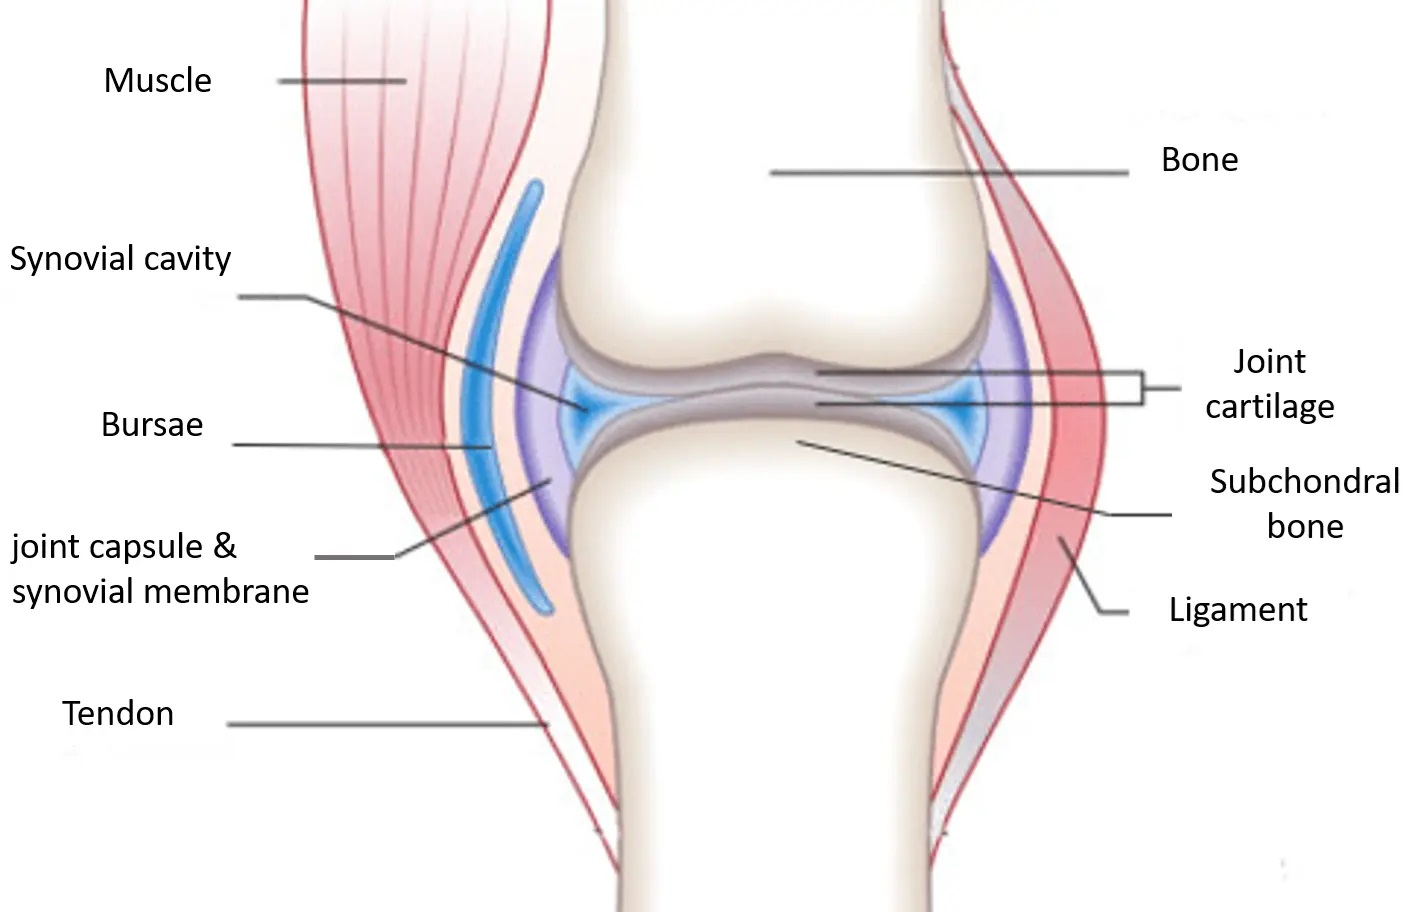
\includegraphics[width=\linewidth,keepaspectratio]{skeleton.jpg} 
		
		{\tiny (Ref: https://www.swiss-alp-health.ch/en/what-is-a-joint/)}
		\end{center}	

    \end{column}
  \end{columns}
\end{frame}



%%%%%%%%%%%%%%%%%%%%%%%%%%%%%%%%%%%%%%%%%%%%%%%%%%%%%%%%%%%
\begin{frame}[fragile]\frametitle{Divisions of the Skeletal System}
\begin{columns}
    \begin{column}[T]{0.5\linewidth}
      \begin{itemize}
		\item Axial Skeleton: Skull, vertebral column, rib cage
			\begin{itemize}
			\item Skull: 23 bones, protects brain, inner ear, eyes
			\item Spine: Made of vertebrae, supports trunk, protects spinal cord
			\item Rib Cage: 12 pairs of ribs, protects lungs and heart
			\end{itemize}

		\item Appendicular Skeleton: Shoulder and pelvic girdles, limbs
			\begin{itemize}
			\item Shoulder Girdle: Shoulder blades, collar bones
			\item Upper Limb: Humerus, radius, ulna, carpals, metacarpals, phalanges
			\item Pelvis: Flat bones from sacrum, base for legs
			\item Lower Limb: Femur, patella, tibia, fibula, tarsals, metatarsals, phalanges
		    \end{itemize}
	  \end{itemize}
    \end{column}
    \begin{column}[T]{0.5\linewidth}
		\begin{center}
		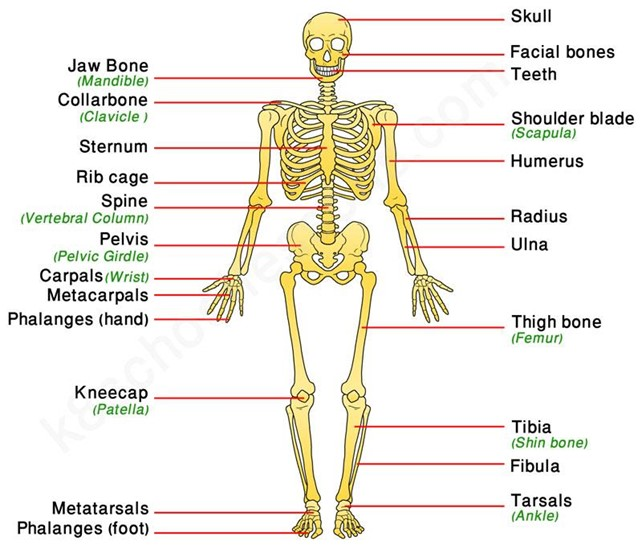
\includegraphics[width=\linewidth,keepaspectratio]{skeleton_divisions.jpg} 
		\end{center}	
    \end{column}
  \end{columns}
\end{frame}

%%%%%%%%%%%%%%%%%%%%%%%%%%%%%%%%%%%%%%%%%%%%%%%%%%%%%%%%%%%
\begin{frame}[fragile]\frametitle{Functions of skeleton system}

\begin{itemize}
\item Structural Framework
\item Support and protection
\item Blood formation
\item Storehouse of minerals
\end{itemize}
	  
\end{frame}


%%%%%%%%%%%%%%%%%%%%%%%%%%%%%%%%%%%%%%%%%%%%%%%%%%%%%%%%%%%
\begin{frame}[fragile]\frametitle{Vertebral Column}
\begin{columns}
    \begin{column}[T]{0.65\linewidth}
      \begin{itemize}
		\item Spine: Strong column of bone from head to lower back
		\item 33 vertebrae joined by cartilage and ligaments
		\item Spinal cord runs through central holes in vertebrae
		\item Vertebrae groups: Cervical (7), Thoracic (12), Lumbar (5)
		\item Sacral (5 fused into 1), Coccygeal (4 fused into 1)
		\item Curvatures: Cervical, Thoracic, Lumbar, Pelvic
		\item Improper posture can exaggerate spinal curves
		\item Kyphosis: Increased thoracic curve
		\item Lordosis: Exaggerated lumbar curve
		\item Scoliosis: Lateral curvature of the spine
		\item Asanas can help correct posture by balancing and strengthening muscles
	  \end{itemize}
    \end{column}
    \begin{column}[T]{0.35\linewidth}
		\begin{center}
		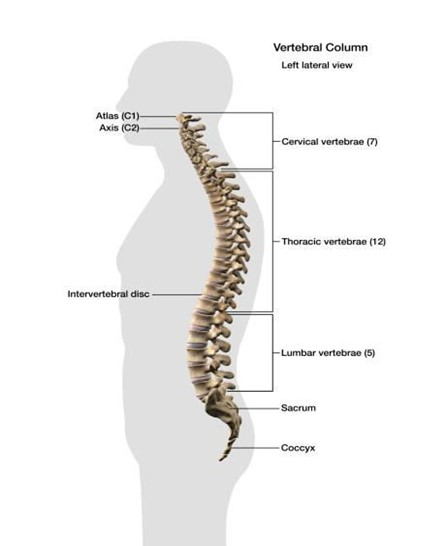
\includegraphics[width=\linewidth,keepaspectratio]{vertebral_column.jpg} 
		\end{center}	
    \end{column}
  \end{columns}
\end{frame}

%%%%%%%%%%%%%%%%%%%%%%%%%%%%%%%%%%%%%%%%%%%%%%%%%%%%%%%%%%%
\begin{frame}[fragile]\frametitle{Types of Spinal Movements}
\begin{columns}
    \begin{column}[T]{0.5\linewidth}
      \begin{itemize}
		\item Flexion: Forward bending; maximal in cervical region (e.g., Paschimotanasana, Padahastasana)
		\item Extension: Back bending (e.g., Bhujangasana, Dhanurasana)
		\item Rotation: Longitudinal twisting; greatest between atlas and axis (e.g., Ardha Matsyendrasana)
		\item Sideways Bending: Maximal in cervical and lumbar regions (e.g., Trikonasana)
		\item Circumduction: Swaying combining all movements (e.g., Chakki Chalavan)
		\item Elongation: Stretching upwards from base of spine (e.g., Tadasana, Urdhvahasta Dandasana)
	  \end{itemize}
    \end{column}
    \begin{column}[T]{0.5\linewidth}
		\begin{center}
		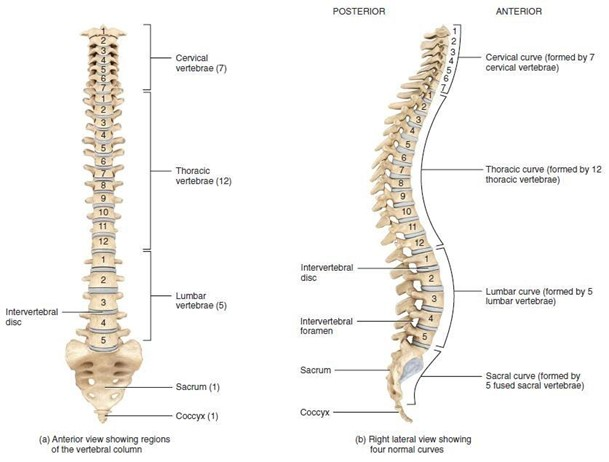
\includegraphics[width=\linewidth,keepaspectratio]{spinal_movements.jpg} 
		\end{center}	
    \end{column}
  \end{columns}
\end{frame}

%%%%%%%%%%%%%%%%%%%%%%%%%%%%%%%%%%%%%%%%%%%%%%%%%%%%%%%%%%%
\begin{frame}[fragile]\frametitle{Types of Joints}

      \begin{itemize}
		\item Joints: Points of contact between two bones
		\item Fibrous Joints: Allow the least movement; e.g., sutures in skull
		\item Cartilaginous Joints: Bones connected by cartilage; e.g., ribs to sternum
		\item Synovial Joints: Highest mobility; coated with cartilage, contain synovial fluid
		\item Fibrous Joints: Immovable parts of the skeletal system
		\item Cartilaginous Joints: Strong but flexible, necessary movement (e.g., breathing)
		\item Synovial Joints: Sealed in fluid-filled joint capsule
		\item Six kinds of synovial joints for various movements
	  \end{itemize}

\end{frame}

%%%%%%%%%%%%%%%%%%%%%%%%%%%%%%%%%%%%%%%%%%%%%%%%%%%%%%%%%%%
\begin{frame}[fragile]\frametitle{Types of Joints}

		\begin{center}
		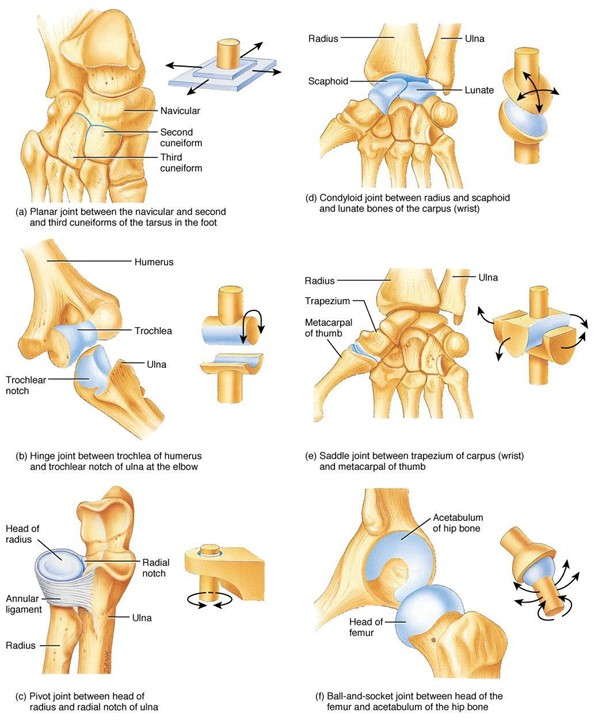
\includegraphics[width=0.5\linewidth,keepaspectratio]{joints.jpg} 
		\end{center}	

\end{frame}

%%%%%%%%%%%%%%%%%%%%%%%%%%%%%%%%%%%%%%%%%%%%%%%%%%%%%%%%%%%
\begin{frame}[fragile]\frametitle{Muscular System Overview}

      \begin{itemize}
		\item Muscles are contractile tissues.
		\item They convert chemical energy into mechanical energy.
		\item Three types of muscles: voluntary, involuntary, cardiac.
		\item Voluntary muscles: consciously controlled.
		\item Involuntary muscles: controlled by autonomic nervous system.
		\item Cardiac muscle: auto rhythmic, contracts without stimulation.
		\item Voluntary muscles aid in walking, balancing, writing.
		\item Involuntary muscles help in digestion, blood flow.
		\item Cardiac muscle is specialized for heart function.
	  \end{itemize}

\end{frame}

%%%%%%%%%%%%%%%%%%%%%%%%%%%%%%%%%%%%%%%%%%%%%%%%%%%%%%%%%%%
\begin{frame}[fragile]\frametitle{Muscular System Overview}

		\begin{center}
		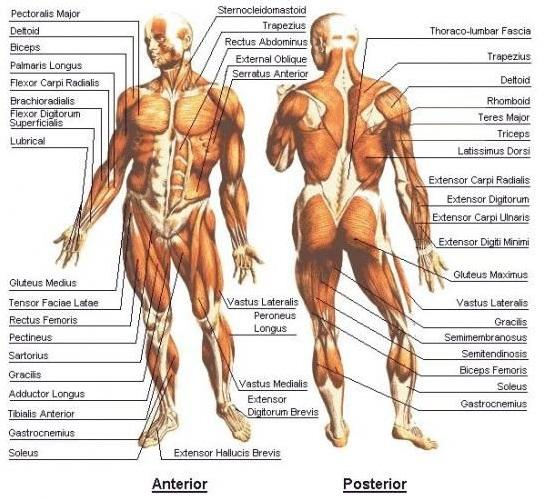
\includegraphics[width=0.6\linewidth,keepaspectratio]{Muscle-chart-showing-the-muscular-system-labeled.jpg}
						
		{\tiny (Ref: https://www.biologyonline.com/dictionary/muscular-system)}			
		\end{center}	

\end{frame}


%%%%%%%%%%%%%%%%%%%%%%%%%%%%%%%%%%%%%%%%%%%%%%%%%%%%%%%%%%%
\begin{frame}[fragile]\frametitle{Functions of Muscular System }

      \begin{itemize}
		\item Production of movement. Maintaining posture against gravity.
		\item Protection of internal organs
		\item Heat production
		\item Store for energy (protein and carbohydrates)
		\item Functioning of internal organs because of involuntary muscles.
	  \end{itemize}

\end{frame}

%%%%%%%%%%%%%%%%%%%%%%%%%%%%%%%%%%%%%%%%%%%%%%%%%%%%%%%%%%%
\begin{frame}[fragile]\frametitle{Muscle Contraction}

      \begin{itemize}
		\item Muscles consist of fibres wrapped in a sheath.
		\item Muscle fibres contain actin (thin) and myosin (thick) filaments.
		\item Filaments overlap to create tension and shorten muscle fibres.
		\item Relaxed muscles: minimal overlap of filaments.
		\item Stimulated muscles: filaments slide and overlap, causing contraction.
		\item Maximal contraction: complete overlap of filaments.
		\item Muscle strength increases through more fibre engagement or efficiency.
		\item Isotonic Contraction: muscle changes shape while load remains constant.
		\item Isometric Contraction: muscle stays same size while load increases.
	  \end{itemize}

\end{frame}

%%%%%%%%%%%%%%%%%%%%%%%%%%%%%%%%%%%%%%%%%%%%%%%%%%%%%%%%%%%
\begin{frame}[fragile]\frametitle{Muscle Contraction}

		\begin{center}
		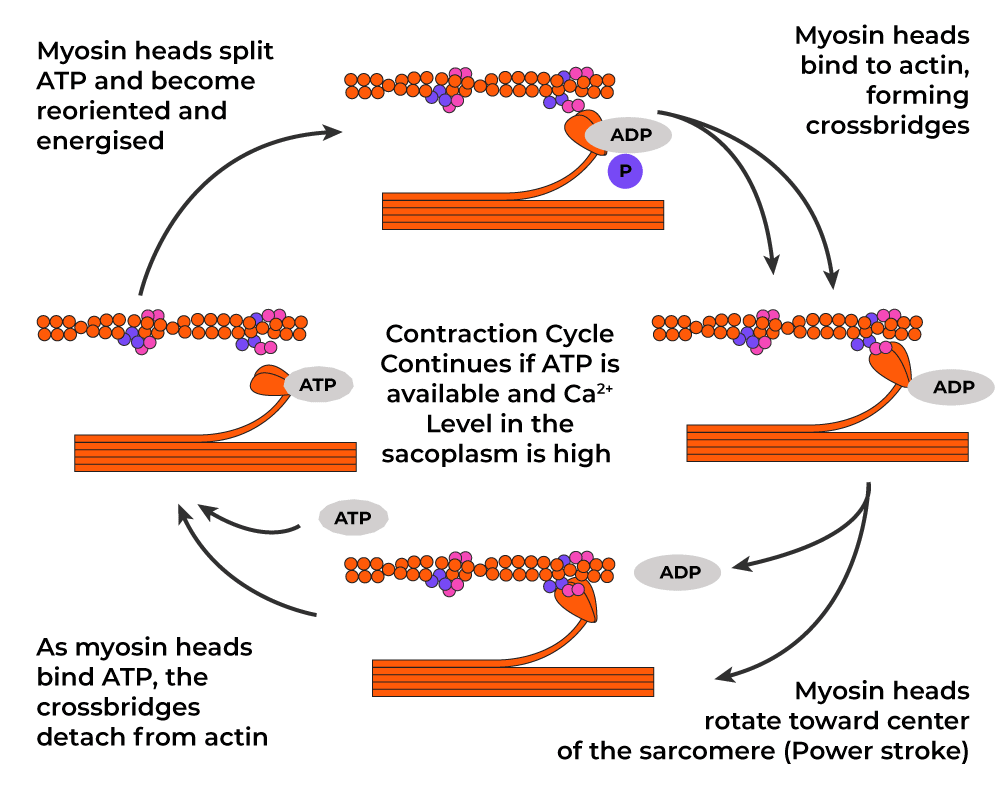
\includegraphics[width=0.8\linewidth,keepaspectratio]{Mechnaism-of-muscle-contrtaction.png}
		
						
		{\tiny (Ref: https://www.geeksforgeeks.org/mechanism-of-muscle-contraction-class-11/)}		
		\end{center}	

\end{frame}

%%%%%%%%%%%%%%%%%%%%%%%%%%%%%%%%%%%%%%%%%%%%%%%%%%%%%%%%%%%
\begin{frame}[fragile]\frametitle{Reflex Action \& Reciprocal Inhibition}

      \begin{itemize}
		\item Motor units: smallest nerve fibre groups in muscles.
		\item Proprioceptors: sensors that send body position info to the brain.
		\item Proprioception aids in posture and coordination.
		\item Stretch reflex: strong contraction when muscle is suddenly lengthened.
		\item Example: back muscles contract when bending forward quickly.
		\item Slow movements support deep breathing.
		\item Reciprocal inhibition: opposing muscles relax when one contracts.
		\item Example: biceps contract, triceps relax.
		\item Ensures smooth and coordinated muscle movements.
	  \end{itemize}

\end{frame}



%%%%%%%%%%%%%%%%%%%%%%%%%%%%%%%%%%%%%%%%%%%%%%%%%%%%%%%%%%%
\begin{frame}[fragile]\frametitle{Reflex Action \& Reciprocal Inhibition}

		\begin{center}
		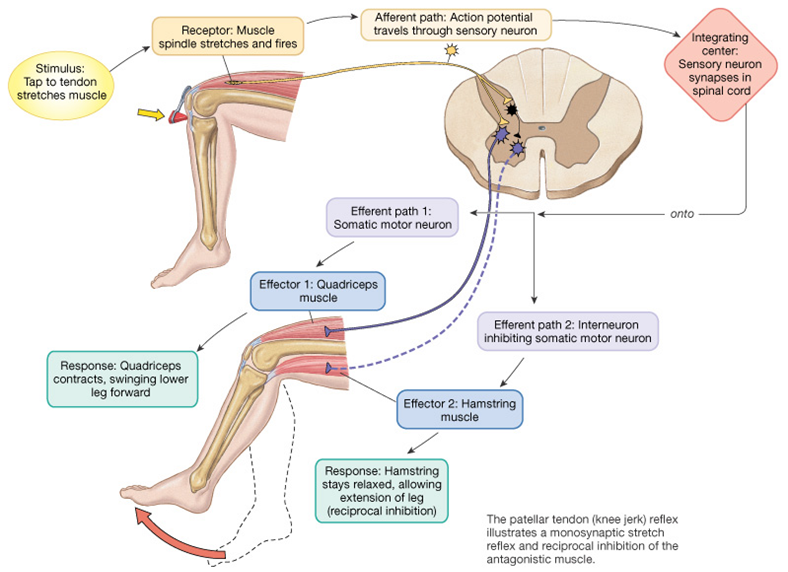
\includegraphics[width=0.8\linewidth,keepaspectratio]{Reciprocal-Inhibition.png}
		
						
		{\tiny (Ref: https://www.corewalking.com/reciprocal-inhibition/)}
		\end{center}	

\end{frame}

%%%%%%%%%%%%%%%%%%%%%%%%%%%%%%%%%%%%%%%%%%%%%%%%%%%%%%%%%%%
\begin{frame}[fragile]\frametitle{Types of Muscle Movements}

      \begin{itemize}
		\item Flexion: Decreases joint angle, e.g., bending the elbow.
		\item Extension: Increases joint angle, e.g., straightening the elbow.
		\item Abduction: Moves bone away from midline, e.g., lifting arms.
		\item Adduction: Moves bone towards midline, e.g., bringing legs together.
		\item Elevation: Movement upward, e.g., shrugging shoulders.
		\item Depression: Movement downward, e.g., lowering shoulders.
		\item Pronation: Palms face down.
		\item Supination: Palms face up.
		\item Rotation: Movement around an axis, e.g., internal or external rotation.
		\item Sphincter opening: Reduces or increases size of an opening.
	  \end{itemize}

  
		{\tiny (Ref: https://med.libretexts.org/Bookshelves/Anatomy\_and\_Physiology/}		
  
\end{frame}

%%%%%%%%%%%%%%%%%%%%%%%%%%%%%%%%%%%%%%%%%%%%%%%%%%%%%%%%%%%
\begin{frame}[fragile]\frametitle{Types of Muscle Movements}

		\begin{center}
		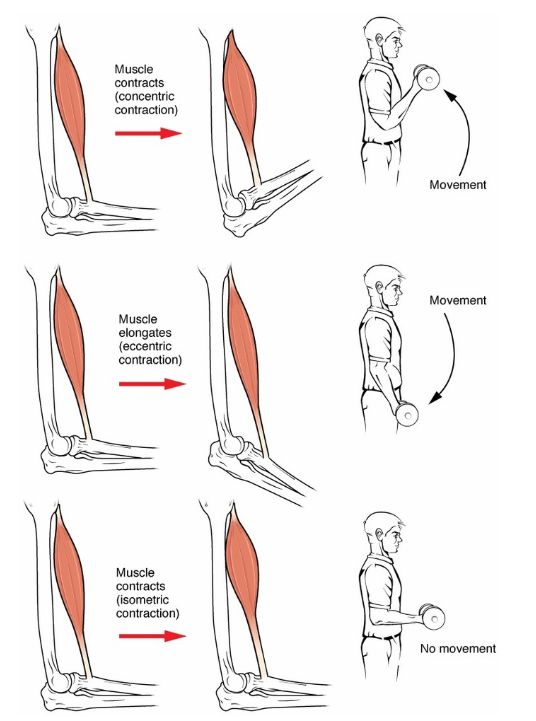
\includegraphics[width=0.4\linewidth,keepaspectratio]{muscletypes}
				
		\end{center}	

  
		{\tiny (Ref: https://med.libretexts.org/Bookshelves/Anatomy\_and\_Physiology/}		
  
\end{frame}

%%%%%%%%%%%%%%%%%%%%%%%%%%%%%%%%%%%%%%%%%%%%%%%%%%%%%%%%%%%
\begin{frame}[fragile]\frametitle{Muscle Breathing}
\begin{columns}
    \begin{column}[T]{0.7\linewidth}
      \begin{itemize}
		\item Muscles need energy for contraction.
		\item Energy comes from glucose metabolism using oxygen.
		\item Aerobic respiration: used in low-intensity, high-volume activities.
		\item Example: marathon running, dance.
		\item Anaerobic respiration: used when oxygen is insufficient or activities are very fast.
		\item Anaerobic respiration produces lactic acid as a byproduct.
		\item Example: weight training, sprints.
		\item Post-exertion: oxygen breaks down lactic acid into water and carbon dioxide.
		\item Oxygen debt: amount of oxygen required to break down lactic acid.
	  \end{itemize}
    \end{column}
    \begin{column}[T]{0.3\linewidth}
		\begin{center}
		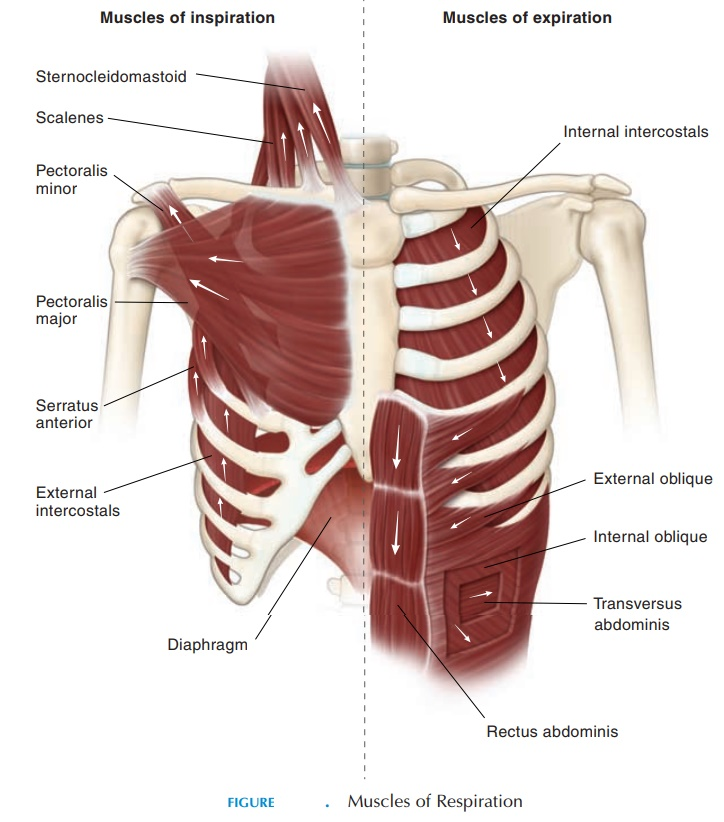
\includegraphics[width=\linewidth,keepaspectratio]{article-Respiration-Muscles-WC1.jpg}
				
		{\tiny (Ref: https://www.brainkart.com/article/Respiration-Muscles\_21121/)}
		\end{center}	
    \end{column}
  \end{columns}
\end{frame}

%%%%%%%%%%%%%%%%%%%%%%%%%%%%%%%%%%%%%%%%%%%%%%%%%%%%%%%%%%%
\begin{frame}[fragile]\frametitle{Cardiovascular System}
\begin{columns}
    \begin{column}[T]{0.6\linewidth}
      \begin{itemize}
		\item Cardiovascular system transports nutrients, gases, waste, hormones.
		\item Blood consists of:
			\begin{itemize}
				\item Plasma (54\% of blood mass)
				\item Red blood cells (45\%)
				\item White blood cells and platelets (1\%)
			\end{itemize}
		\item Red Blood Cells (RBCs): Transport oxygen and carbon dioxide.
		\item RBCs produced in bone marrow, lifespan ~120 days.
		\item Anaemia: Condition when RBC count falls below 30\%.
		\item White Blood Cells (WBCs): Provide immunity, lifespan 30 hours to 25 days.
		\item Platelets: Prevent bleeding by sticking to damaged vessels.
		\item Platelets' average lifespan is 4 days.
	  \end{itemize}
    \end{column}
    \begin{column}[T]{0.4\linewidth}
		\begin{center}
		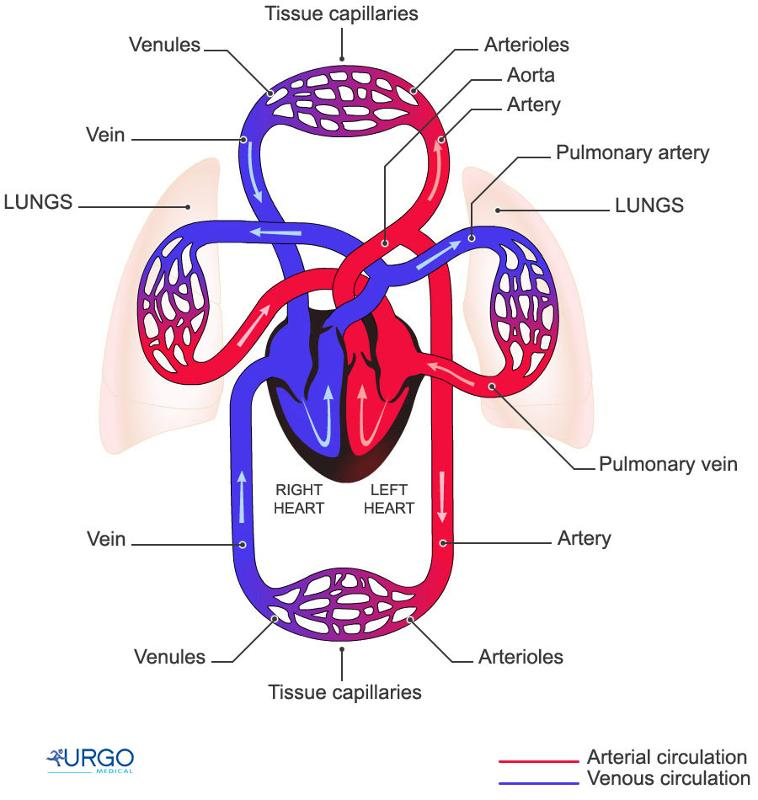
\includegraphics[width=\linewidth,keepaspectratio]{CardiovascularSystem.jpg}
		
				
		{\tiny (Ref: https://www.meresearch.org.uk/taking-heart-1/)}		
		\end{center}	
    \end{column}
  \end{columns}
\end{frame}

%%%%%%%%%%%%%%%%%%%%%%%%%%%%%%%%%%%%%%%%%%%%%%%%%%%%%%%%%%%
\begin{frame}[fragile]\frametitle{Blood Vessels \& Heart}

      \begin{itemize}
		\item Blood vessels transport blood throughout the body.
		\item Arteries carry blood away from the heart.
		\item Arteries branch into arterioles, then into capillaries for nutrient exchange.
		\item Capillaries converge into venules, which merge into veins.
		\item Veins carry blood back to the heart.
		\item Systemic circulation: blood flow to and from the body.
		\item Pulmonary circulation: blood flow to and from the lungs.
		\item Heart: muscular organ that pumps blood.
		\item Heart has 4 chambers: right atrium, left atrium, right ventricle, left ventricle.
		\item Atria receive blood; ventricles pump it out.
		\item Valves prevent backflow: tricuspid (right), bicuspid/mitral (left).
	  \end{itemize}
  
\end{frame}

%%%%%%%%%%%%%%%%%%%%%%%%%%%%%%%%%%%%%%%%%%%%%%%%%%%%%%%%%%%
\begin{frame}[fragile]\frametitle{Blood Vessels \& Heart}

		\begin{center}
		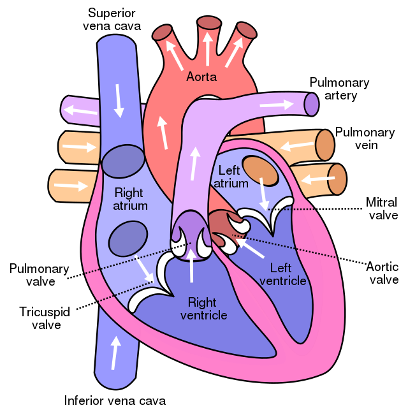
\includegraphics[width=0.6\linewidth,keepaspectratio]{Heart-diagram.png}
				
		{\tiny (Ref: https://www.meresearch.org.uk/taking-heart-1/)}
		\end{center}	

\end{frame}


%%%%%%%%%%%%%%%%%%%%%%%%%%%%%%%%%%%%%%%%%%%%%%%%%%%%%%%%%%%
\begin{frame}[fragile]\frametitle{Functions of Muscular System }

      \begin{itemize}
		\item Transport, blood circulation.
		\item Protection, immunity.
		\item Homeostasis.
	  \end{itemize}

\end{frame}

%%%%%%%%%%%%%%%%%%%%%%%%%%%%%%%%%%%%%%%%%%%%%%%%%%%%%%%%%%%
\begin{frame}[fragile]\frametitle{Respiratory System}

      \begin{itemize}
		\item Respiration: Exchange of oxygen and carbon dioxide.
		\item At pulmonary level: Oxygen diffuses into capillaries, $CO_2$ into alveoli.
		\item At systemic level: Gas exchange occurs in capillaries near cells.
		\item Respiratory tract: Pathway for air to and from the lungs.
		\item Nose: Filters, warms, and moistens air; sense organ for smell.
		\item Pharynx: Passage from mouth and nose; connects to larynx.
		\item Larynx: Voice box; produces sound.
		\item Trachea: Windpipe; held open by cartilage rings.
		\item Bronchi, bronchioles, alveoli: Air passage branches ending in alveoli for gas exchange.
		\item Lungs: Triangular air sacs; two on the left (2 lobes), three on the right.
		\item Respiratory mucosa: Secretes mucus, traps irritants, and moves mucus to pharynx.
		\item Sinuses: Air-filled spaces around nasal cavity; prone to blockage and sinusitis.
	  \end{itemize}

\end{frame}

%%%%%%%%%%%%%%%%%%%%%%%%%%%%%%%%%%%%%%%%%%%%%%%%%%%%%%%%%%%
\begin{frame}[fragile]\frametitle{Respiratory System}
\
		\begin{center}
		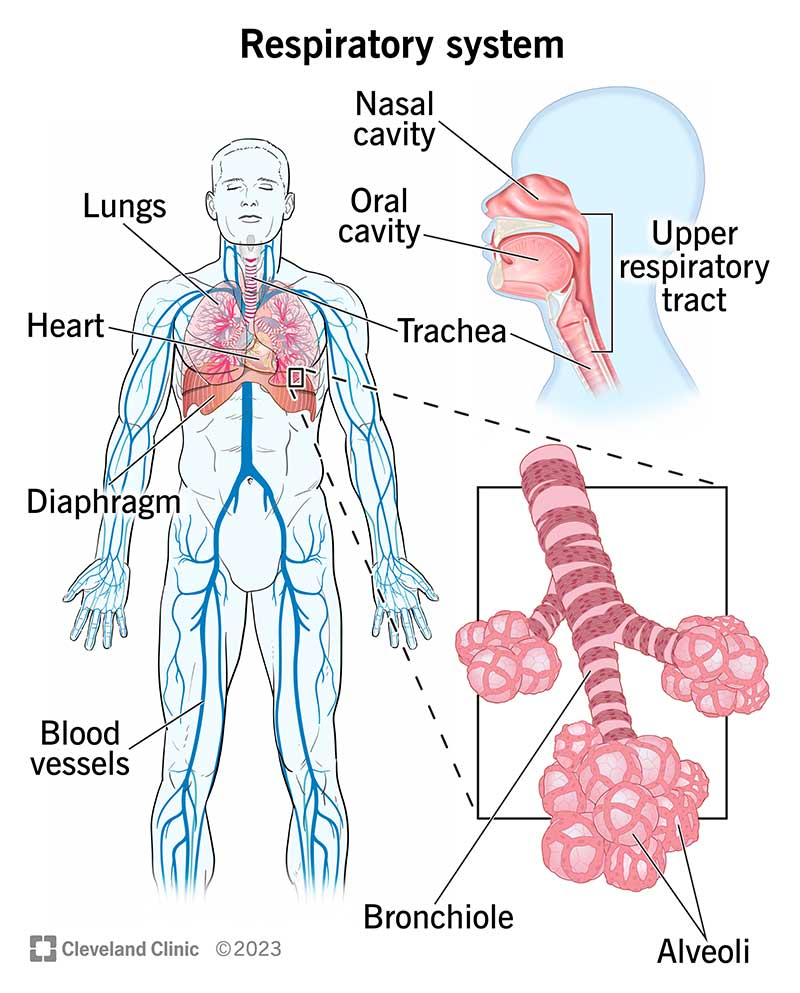
\includegraphics[width=0.45\linewidth,keepaspectratio]{respiratory-system.jpg}
		\end{center}	

\end{frame}
%%%%%%%%%%%%%%%%%%%%%%%%%%%%%%%%%%%%%%%%%%%%%%%%%%%%%%%%%%%
\begin{frame}[fragile]\frametitle{Functions of Muscular System }

      \begin{itemize}
		\item Exchange of gases
		\item Maintaining pH balance
		\item Speech production.
	  \end{itemize}

\end{frame}
	
%%%%%%%%%%%%%%%%%%%%%%%%%%%%%%%%%%%%%%%%%%%%%%%%%%%%%%%%%%%
\begin{frame}[fragile]\frametitle{Muscles of Respiration}
\begin{columns}
    \begin{column}[T]{0.5\linewidth}
      \begin{itemize}
		\item Diaphragm: Dome-shaped muscle below lungs; separates chest and abdominal cavities.
		\item Intercostal Muscles: Located between ribs; lift rib cage for inhalation, lower it for exhalation.
		\item Accessory Muscles: Neck muscles attached to collarbone; assist in clavicular breathing.
		\item Muscles of Expiration: Abdominal muscles; used for forceful exhalation.
	  \end{itemize}
    \end{column}
    \begin{column}[T]{0.5\linewidth}
		\begin{center}
		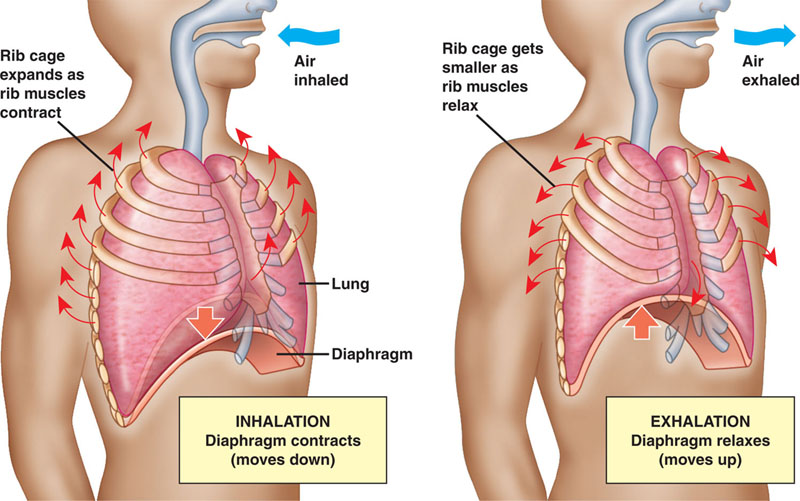
\includegraphics[width=\linewidth,keepaspectratio]{breathing.jpg}
		
		{\tiny (Ref: https://step1.medbullets.com/respiratory/117007/muscles-of-respiration)}
		\end{center}	
    \end{column}
  \end{columns}
\end{frame}

%%%%%%%%%%%%%%%%%%%%%%%%%%%%%%%%%%%%%%%%%%%%%%%%%%%%%%%%%%%
\begin{frame}[fragile]\frametitle{Digestive System}

      \begin{itemize}
		\item Digestion: Breaking down complex molecules into simpler ones (glucose, fatty acids, amino acids).
		\item Alimentary Canal: 12 meters long muscular tube with mucosal lining.
		\item Food movement: By peristalsis (wave-like contractions).
		\item Mouth: Mechanical breakdown (chewing) and initial carbohydrate digestion by saliva.
		\item Oesophagus: Connects mouth to stomach; no digestion or absorption.
		\item Stomach: Mechanical breakdown and initial chemical digestion of proteins, fats, and milk. No absorption; secretes hydrochloric acid.
		\item Small Intestine: 6m long, divided into duodenum, jejunum, ileum; digestion and absorption of nutrients. Villi increase absorption surface area.
		\item Large Intestine: Absorbs water, forms feces; consists of ascending, transverse, descending colon, rectum, and anus.
	  \end{itemize}

\end{frame}

%%%%%%%%%%%%%%%%%%%%%%%%%%%%%%%%%%%%%%%%%%%%%%%%%%%%%%%%%%%
\begin{frame}[fragile]\frametitle{Digestive System}

		\begin{center}
		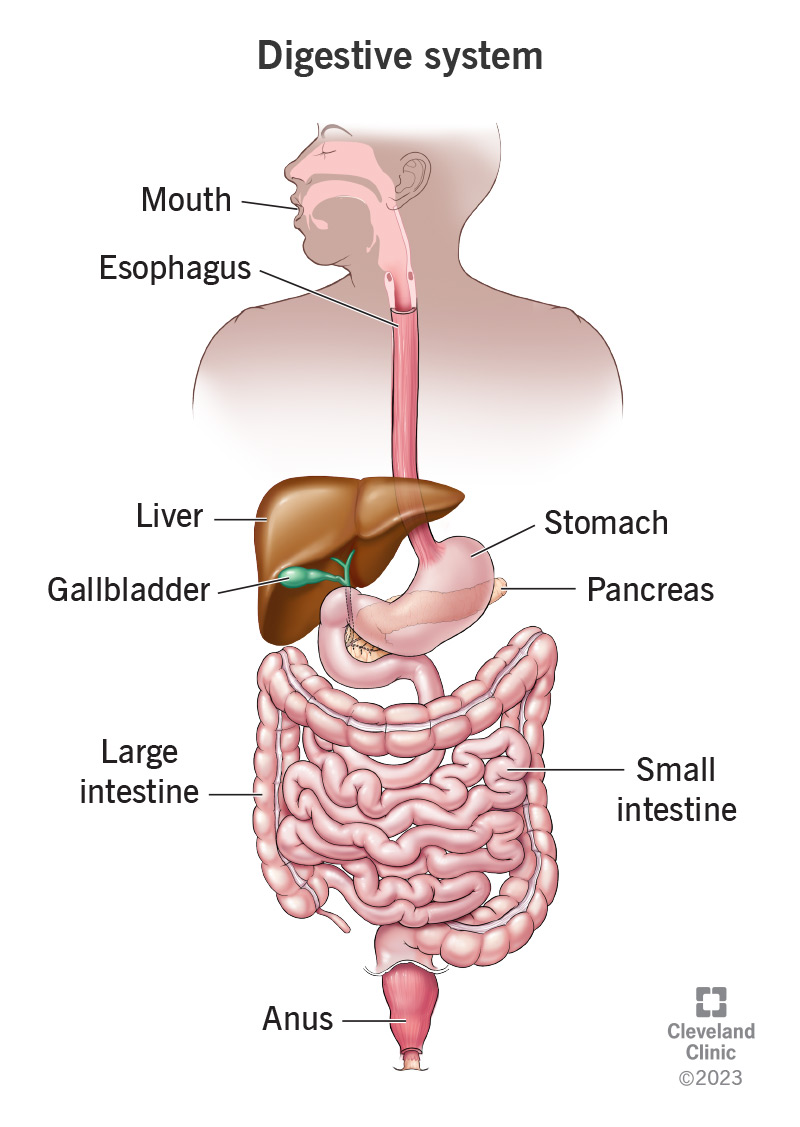
\includegraphics[width=0.45\linewidth,keepaspectratio]{digestive-system.jpg}
		
		{\tiny (Ref: https://my.clevelandclinic.org/health/body/7041-digestive-system)}
		\end{center}	

\end{frame}

%%%%%%%%%%%%%%%%%%%%%%%%%%%%%%%%%%%%%%%%%%%%%%%%%%%%%%%%%%%
\begin{frame}[fragile]\frametitle{Excretory System}
\begin{columns}
    \begin{column}[T]{0.5\linewidth}
      \begin{itemize}
		\item Kidneys: Bean-shaped organs that filter blood; contain ~1 million nephrons each.
		\item Ureters: Smooth muscle tubes that transport urine from kidneys to bladder via peristalsis.
		\item Urinary Bladder: Hollow organ that stores urine; holds 300-500 ml before the urge to urinate.
		\item Urethra: Tube connecting bladder to external orifice for urine expulsion.
	  \end{itemize}
    \end{column}
    \begin{column}[T]{0.5\linewidth}
		\begin{center}
		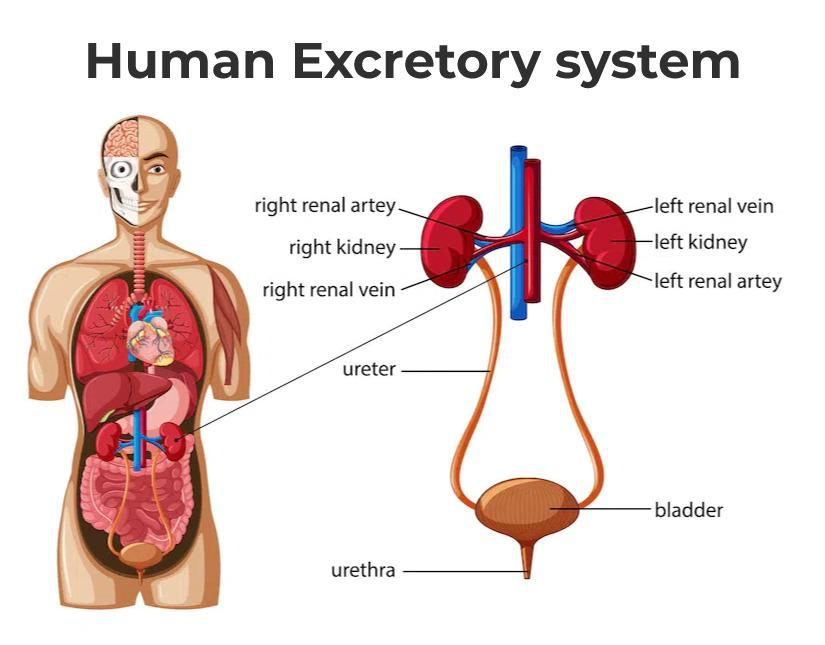
\includegraphics[width=\linewidth,keepaspectratio]{Human-Excretory-System.jpg}
		
		{\tiny (Ref: https://www.geeksforgeeks.org/diagram-of-excretory-system/)}
		\end{center}	
    \end{column}
  \end{columns}
\end{frame}
%%%%%%%%%%%%%%%%%%%%%%%%%%%%%%%%%%%%%%%%%%%%%%%%%%%%%%%%%%%
\begin{frame}[fragile]\frametitle{Functions of Muscular System }

      \begin{itemize}
		\item Eliminate waste from the body.
		\item Regulate blood volume and blood pressure.
		\item Control levels of electrolytes and metabolites
		\item Regulate blood pH.

	  \end{itemize}

\end{frame}

%%%%%%%%%%%%%%%%%%%%%%%%%%%%%%%%%%%%%%%%%%%%%%%%%%%%%%%%%%%
\begin{frame}[fragile]\frametitle{Endocrine System}
\begin{columns}
    \begin{column}[T]{0.5\linewidth}
      \begin{itemize}
		\item Endocrine System: Regulates body activities through hormones.
		\item Hormones: Chemical regulators secreted into the blood.
		\item Secreted directly into blood; act on specific target organs.
		\item Produced in small quantities; not stored in the body.
		\item Types: Water-soluble proteins and amines, lipid-soluble steroids.
		\item Imbalance: Excess or deficiency can lead to serious health issues.
	  \end{itemize}
    \end{column}
    \begin{column}[T]{0.5\linewidth}
		\begin{center}
		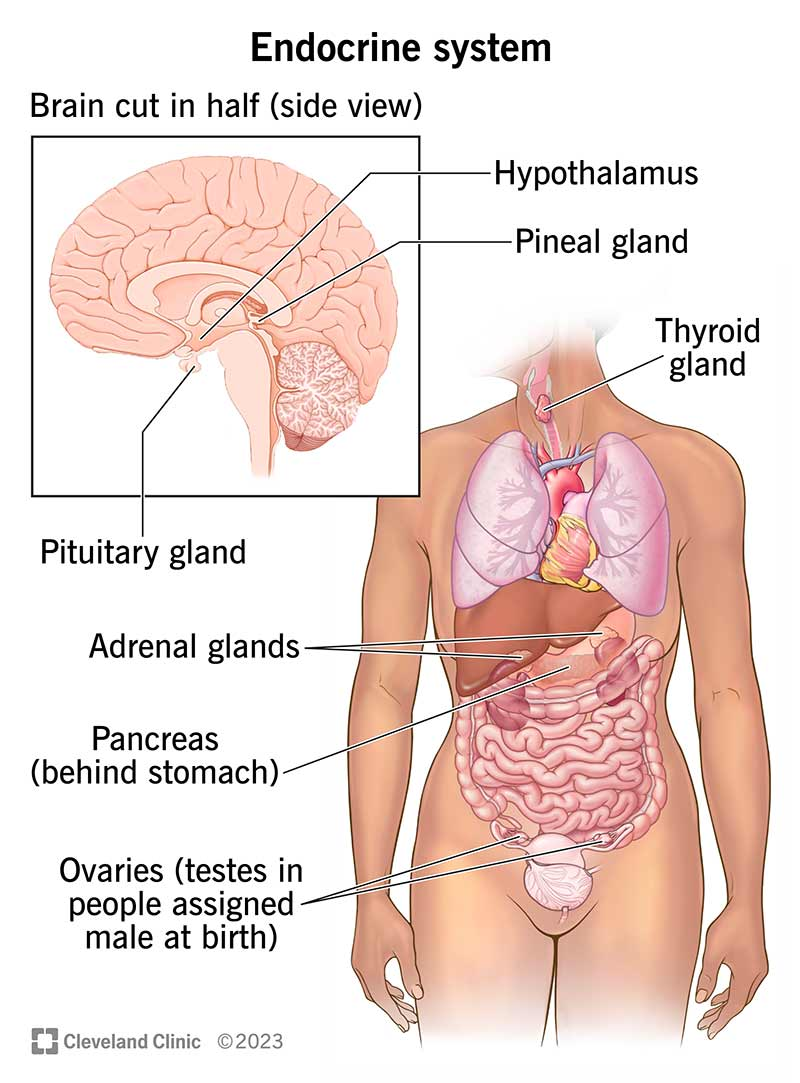
\includegraphics[width=0.8\linewidth,keepaspectratio]{endocrine-system.jpg}
		\end{center}	
    \end{column}
  \end{columns}
\end{frame}

%%%%%%%%%%%%%%%%%%%%%%%%%%%%%%%%%%%%%%%%%%%%%%%%%%%%%%%%%%%
\begin{frame}[fragile]\frametitle{Endocrine Glands: Hypothalamus and Pituitary}

      \begin{itemize}
		\item Hypothalamus: Directs pituitary gland.
		  \begin{itemize}
		    \item Releasing Hormone (RH): Stimulates pituitary hormone release.
		    \item Inhibiting Hormone (IH): Stops pituitary hormone release.
		  \end{itemize}
		\item Pituitary Gland: Master gland; regulates other endocrine glands.
		  \begin{itemize}
		    \item Growth Hormone (GH): Promotes growth.
		    \item Follicle Stimulating Hormone (FSH): Stimulates egg and sperm formation.
		    \item Luteinizing Hormone (LH): Stimulates corpus luteum and hormone production.
		    \item Prolactin: Milk secretion.
		    \item Thyroid Stimulating Hormone (TSH): Stimulates thyroid.
		    \item Adrenocorticotropic Hormone (ACTH): Stimulates adrenal glands.
		    \item Antidiuretic Hormone (ADH): Increases water reabsorption.
		    \item Oxytocin: Uterine contractions.
		  \end{itemize}
	  \end{itemize}

\end{frame}

%%%%%%%%%%%%%%%%%%%%%%%%%%%%%%%%%%%%%%%%%%%%%%%%%%%%%%%%%%%
\begin{frame}[fragile]\frametitle{Endocrine Glands: Hypothalamus and Pituitary}

		\begin{center}
		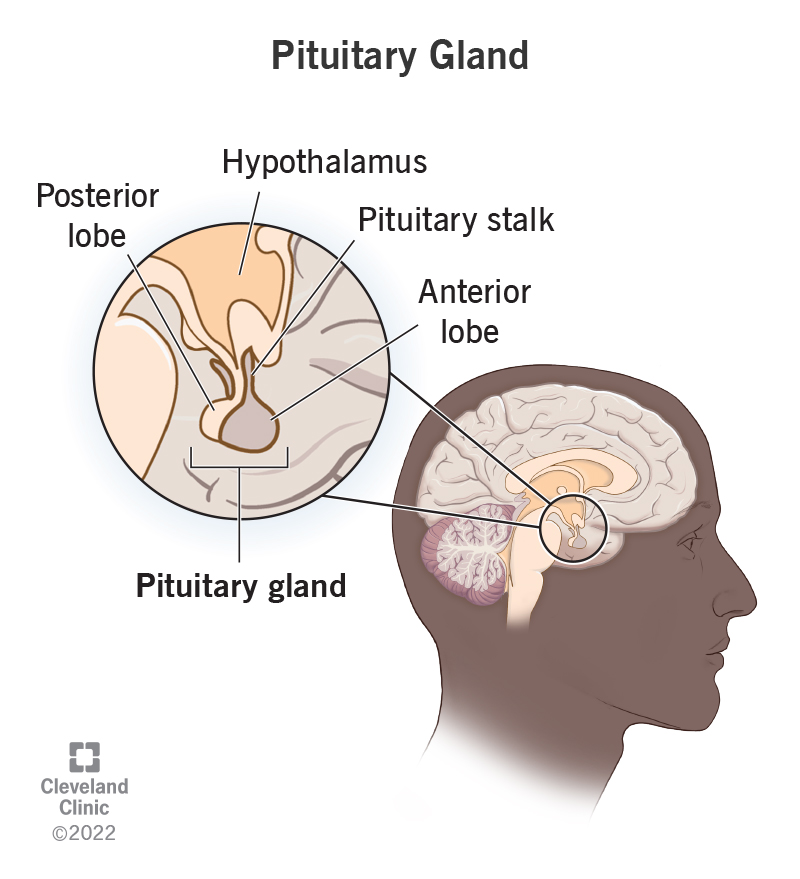
\includegraphics[width=0.5\linewidth,keepaspectratio]{pituitary-gland.jpg}
		
		{\tiny (Ref: https://my.clevelandclinic.org/health/body/21459-pituitary-gland)}
		\end{center}	

\end{frame}


%%%%%%%%%%%%%%%%%%%%%%%%%%%%%%%%%%%%%%%%%%%%%%%%%%%%%%%%%%%
\begin{frame}[fragile]\frametitle{Endocrine Glands: Pineal, Thyroid, and Parathyroid}
\begin{columns}
    \begin{column}[T]{0.5\linewidth}
      \begin{itemize}
		\item Pineal Gland: Produces melatonin; regulates sleep patterns.
		\item Thyroid: Produces thyroxin and calcitonin; regulates metabolism and calcium.
		\item Parathyroid Glands: Regulates calcium metabolism.
	  \end{itemize}
    \end{column}
    \begin{column}[T]{0.5\linewidth}
		\begin{center}
		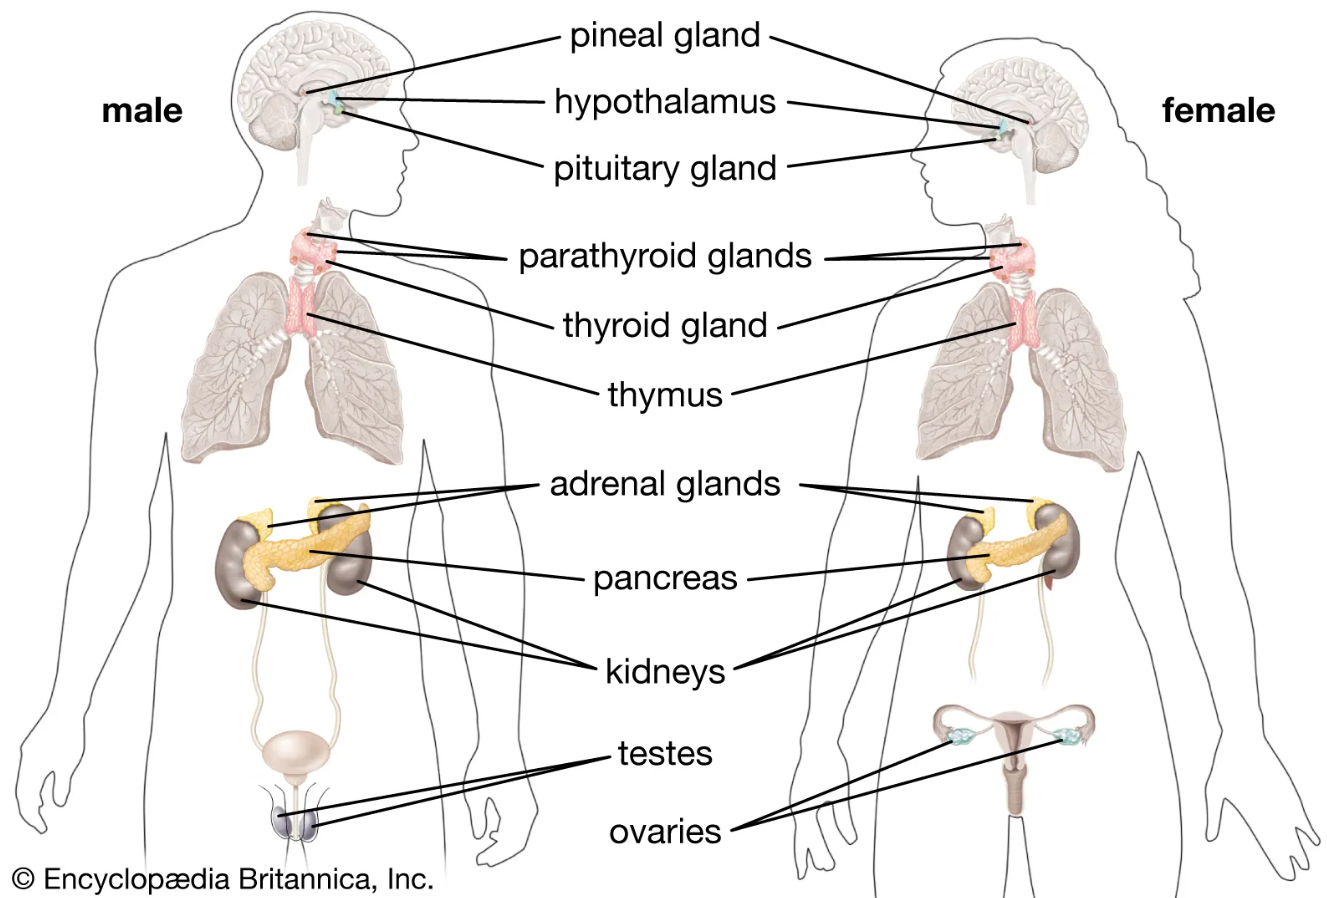
\includegraphics[width=\linewidth,keepaspectratio]{endocrine}
		\end{center}	
    \end{column}
  \end{columns}
\end{frame}

%%%%%%%%%%%%%%%%%%%%%%%%%%%%%%%%%%%%%%%%%%%%%%%%%%%%%%%%%%%
\begin{frame}[fragile]\frametitle{Overview of Reproductive System}
\begin{columns}
    \begin{column}[T]{0.5\linewidth}
      \begin{itemize}
		\item Essential for species survival.
		\item Humans procreate via sexual reproduction.
		\item Gametes: sperm (male) and egg (female).
		\item Fertilization forms a zygote.
		\item Zygote develops into an embryo, then a fetus.
	  \end{itemize}
    \end{column}
    \begin{column}[T]{0.5\linewidth}
		\begin{center}
		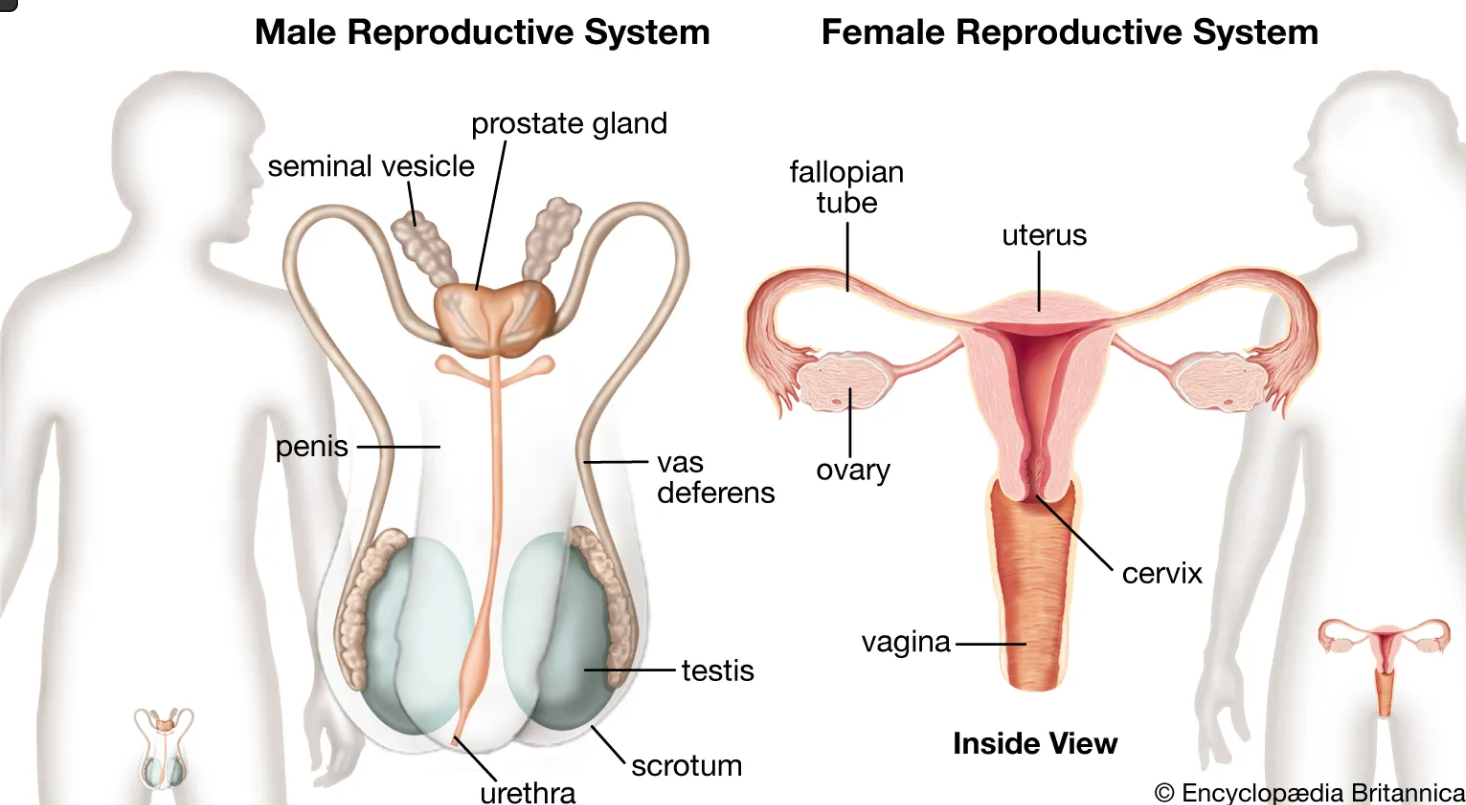
\includegraphics[width=\linewidth,keepaspectratio]{reprosys}

		
		{\tiny (Ref: https://www.britannica.com/science/human-reproductive-system)}		
		\end{center}	
    \end{column}
  \end{columns}
\end{frame}

%%%%%%%%%%%%%%%%%%%%%%%%%%%%%%%%%%%%%%%%%%%%%%%%%%%%%%%%%%%
\begin{frame}[fragile]\frametitle{Male Reproductive System}
\begin{columns}
    \begin{column}[T]{0.5\linewidth}
      \begin{itemize}
		\item Testes: Oval-shaped, produce sperm.
		\item Scrotum: Sac that holds testes.
		\item Seminal Vesicles: Produce seminal fluid.
		\item Prostate Gland: Adds fluids to semen.
		\item Penis: Passes urine and semen.
	  \end{itemize}
    \end{column}
    \begin{column}[T]{0.5\linewidth}
		\begin{center}
		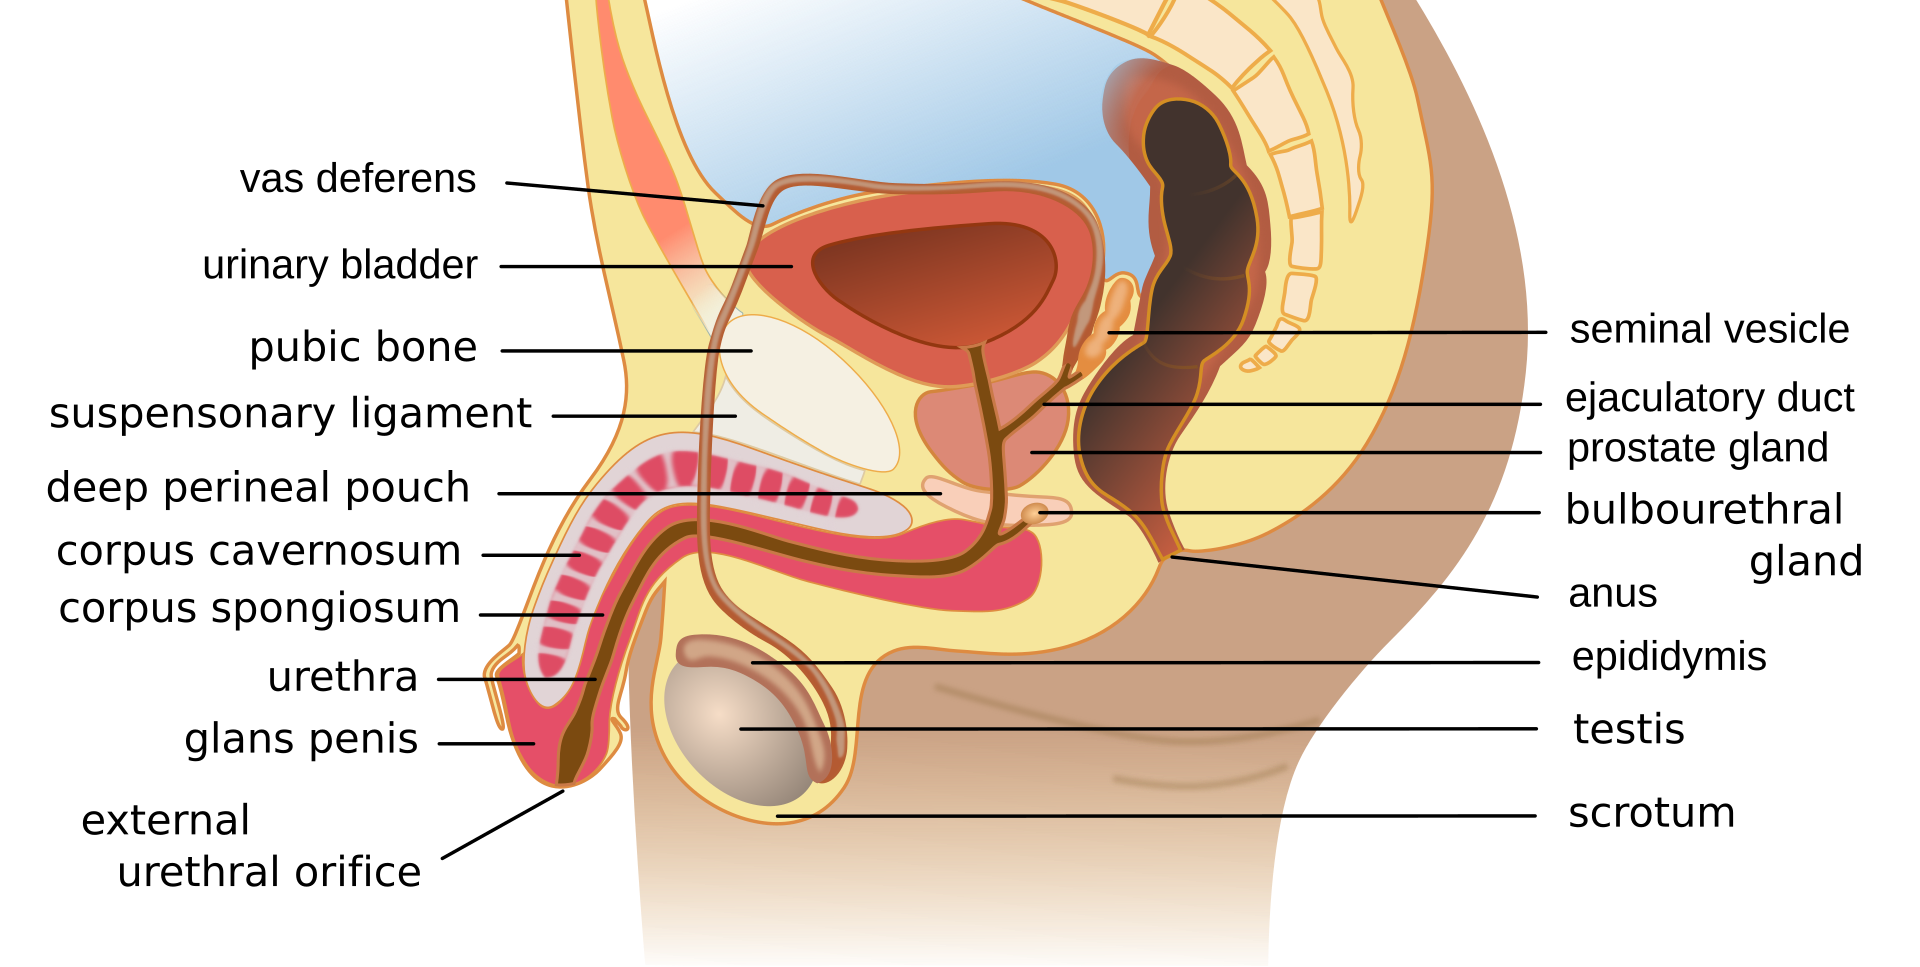
\includegraphics[width=\linewidth,keepaspectratio]{Human_male_reproductive_system_en.svg.png}
		
		{\tiny (Ref: https://simple.wikipedia.org/wiki/Male\_reproductive\_system)}
		\end{center}	
    \end{column}
  \end{columns}
\end{frame}

%%%%%%%%%%%%%%%%%%%%%%%%%%%%%%%%%%%%%%%%%%%%%%%%%%%%%%%%%%%
\begin{frame}[fragile]\frametitle{Female Reproductive System}
\begin{columns}
    \begin{column}[T]{0.5\linewidth}
      \begin{itemize}
		\item Key organs: Ovaries, oviducts, uterus, vagina.
		\item Functions: Egg production, fertilization, embryo development.
		\item Ovaries: Produce and mature eggs.
		\item Oviducts: Site of fertilization.
		\item Uterus: Houses and nurtures the embryo.
	  \end{itemize}
    \end{column}
    \begin{column}[T]{0.5\linewidth}
		\begin{center}
		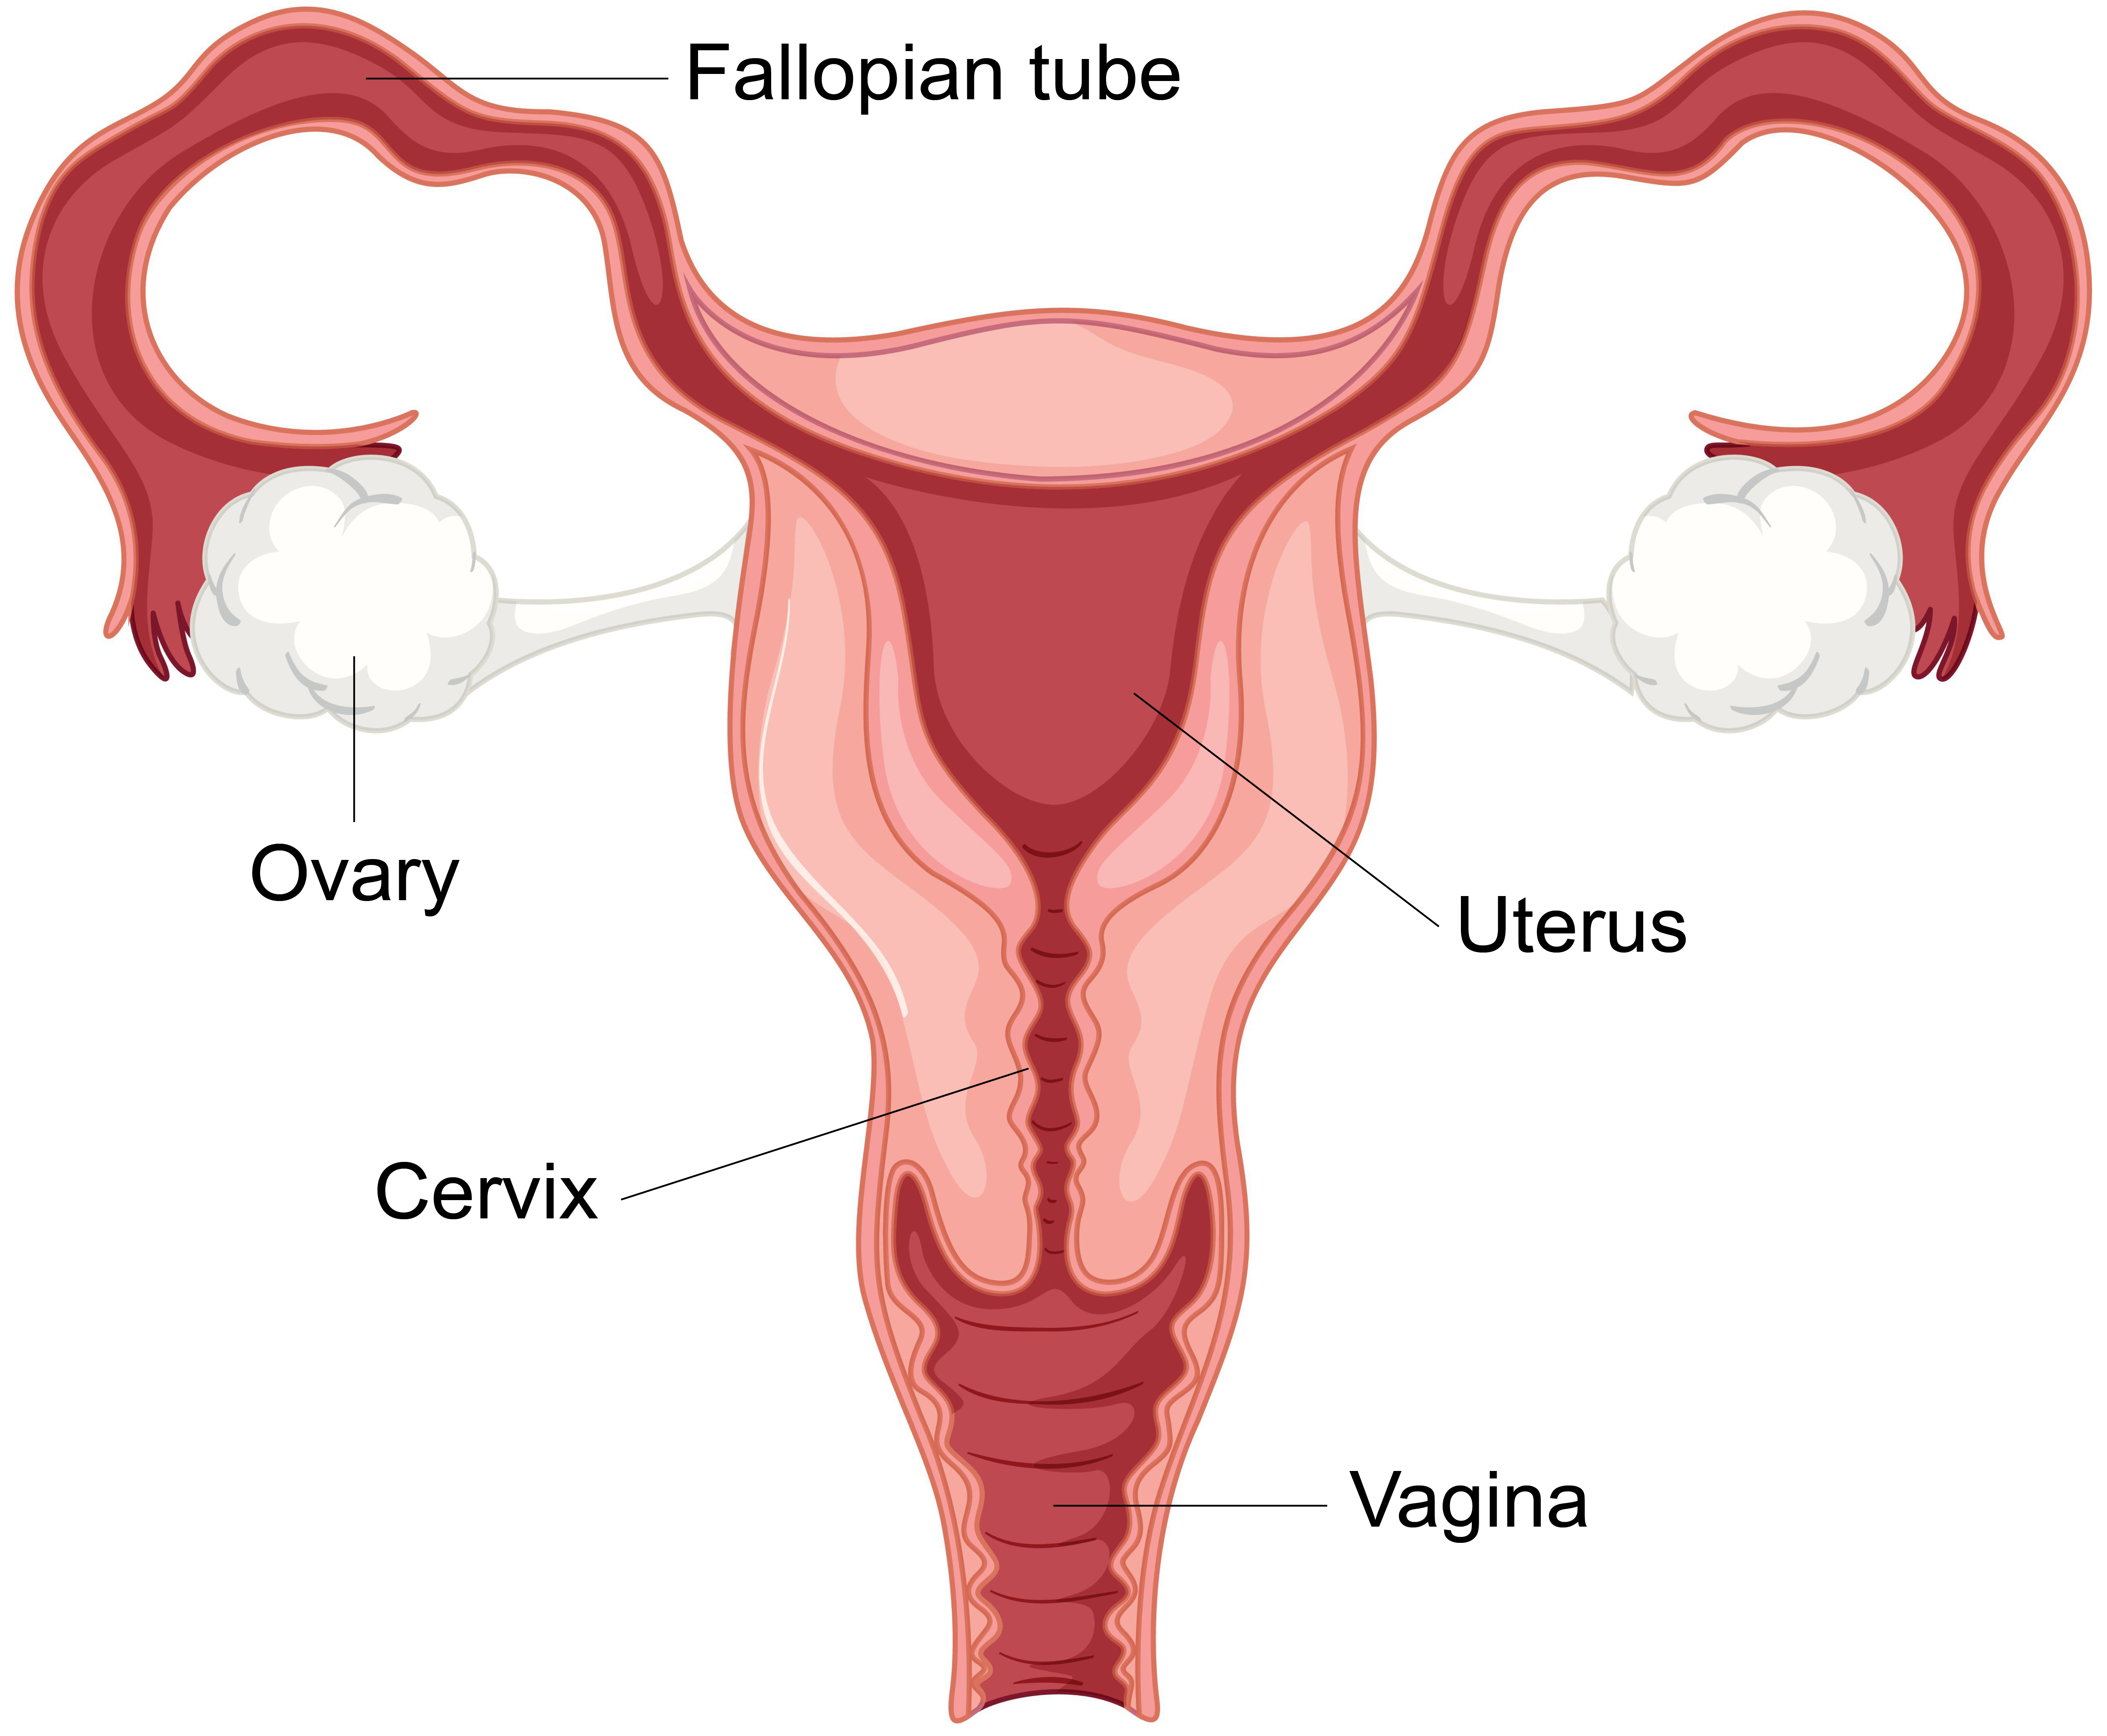
\includegraphics[width=\linewidth,keepaspectratio]{female-reproductive-system.jpg}
		
		{\tiny (Ref: https://www.healthdirect.gov.au/female-reproductive-system)}		
		\end{center}	
    \end{column}
  \end{columns}
\end{frame}

%%%%%%%%%%%%%%%%%%%%%%%%%%%%%%%%%%%%%%%%%%%%%%%%%%%%%%%%%%%
\begin{frame}[fragile]\frametitle{Overview of Nervous System}
\begin{columns}
    \begin{column}[T]{0.5\linewidth}
      \begin{itemize}
		\item Coordinates and controls body actions.
		\item Neuron: basic functional unit.
		\item Consists of CNS and PNS.
		\item CNS: Brain and spinal cord.
		\item PNS: Nerves connecting CNS to body.
	  \end{itemize}
    \end{column}
    \begin{column}[T]{0.5\linewidth}
		\begin{center}
		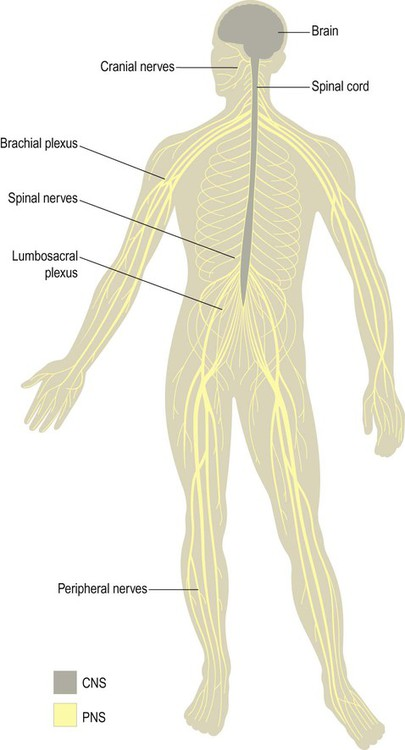
\includegraphics[width=0.6\linewidth,keepaspectratio]{overview_nervious_system}
		
		{\tiny (Ref: https://neupsykey.com/overview-of-the-nervous-system/)}
		
		\end{center}	
    \end{column}
  \end{columns}
\end{frame}

%%%%%%%%%%%%%%%%%%%%%%%%%%%%%%%%%%%%%%%%%%%%%%%%%%%%%%%%%%%
\begin{frame}[fragile]\frametitle{Central Nervous System: Brain}
\begin{columns}
    \begin{column}[T]{0.5\linewidth}
      \begin{itemize}
		\item Brain: Protected by skull and meninges.
		\item Cerebrum: Largest part, divided into lobes.
		\item Cerebellum: Coordinates movements and balance.
		\item Medulla Oblongata: Controls vital functions.
		\item Diencephalon: Includes hypothalamus and thalamus.
	  \end{itemize}
    \end{column}
    \begin{column}[T]{0.5\linewidth}
		\begin{center}
		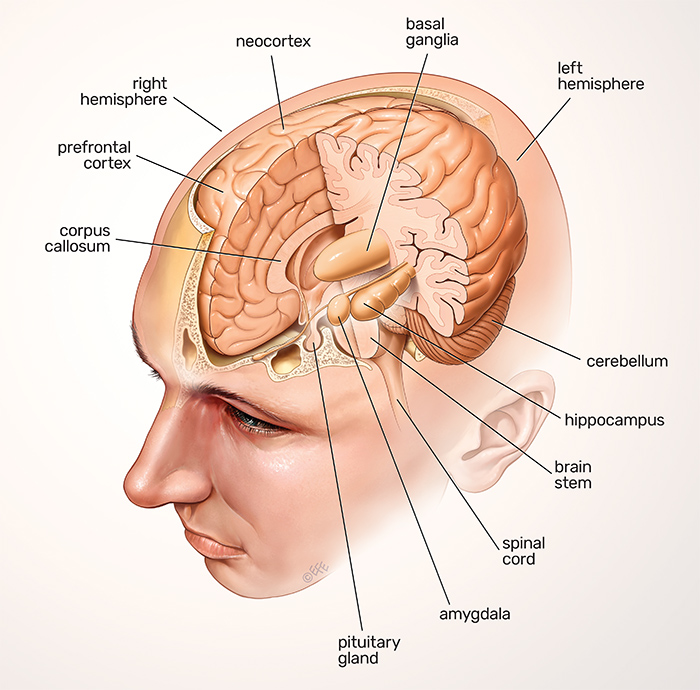
\includegraphics[width=\linewidth,keepaspectratio]{Basic-brain-anatomy.jpg}
		
		{\tiny (Ref: https://qbi.uq.edu.au/brain/brain-anatomy/central-nervous-system-brain-and-spinal-cord)}
		
		\end{center}	
    \end{column}
  \end{columns}
\end{frame}

%%%%%%%%%%%%%%%%%%%%%%%%%%%%%%%%%%%%%%%%%%%%%%%%%%%%%%%%%%%
\begin{frame}[fragile]\frametitle{Central Nervous System: Spinal Cord}
\begin{columns}
    \begin{column}[T]{0.5\linewidth}
      \begin{itemize}
		\item Extends from medulla oblongata to lumbar vertebra.
		\item Covered by meninges.
		\item Facilitates reflex actions.
		\item Conduction of sensory and motor impulses.
		\item Key role in communication between brain and body.
	  \end{itemize}
    \end{column}
    \begin{column}[T]{0.5\linewidth}
		\begin{center}
		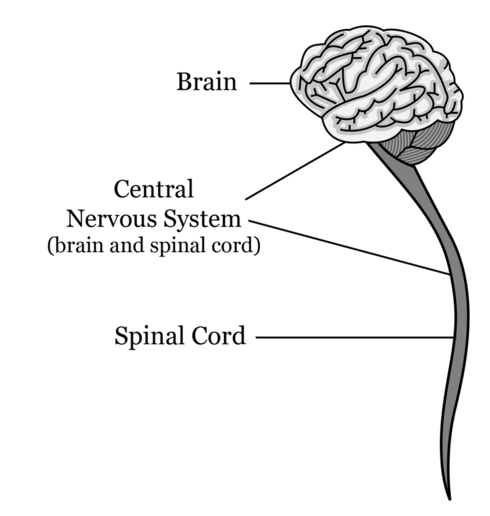
\includegraphics[width=\linewidth,keepaspectratio]{Spinal_chord}
		
		{\tiny (Ref: https://www.ck12.org/biology/central-nervous-system/lesson/central-nervous-system-ms-ls/)}
		\end{center}	
    \end{column}
  \end{columns}
\end{frame}

%%%%%%%%%%%%%%%%%%%%%%%%%%%%%%%%%%%%%%%%%%%%%%%%%%%%%%%%%%%
\begin{frame}[fragile]\frametitle{Peripheral Nervous System: Overview}
\begin{columns}
    \begin{column}[T]{0.5\linewidth}
      \begin{itemize}
		\item Includes all nerves outside CNS.
		\item Connects CNS to limbs and organs.
		\item Divided into Somatic and Autonomic systems.
		\item Somatic: Controls voluntary movements.
		\item Autonomic: Regulates involuntary functions.
	  \end{itemize}
    \end{column}
    \begin{column}[T]{0.5\linewidth}
		\begin{center}
		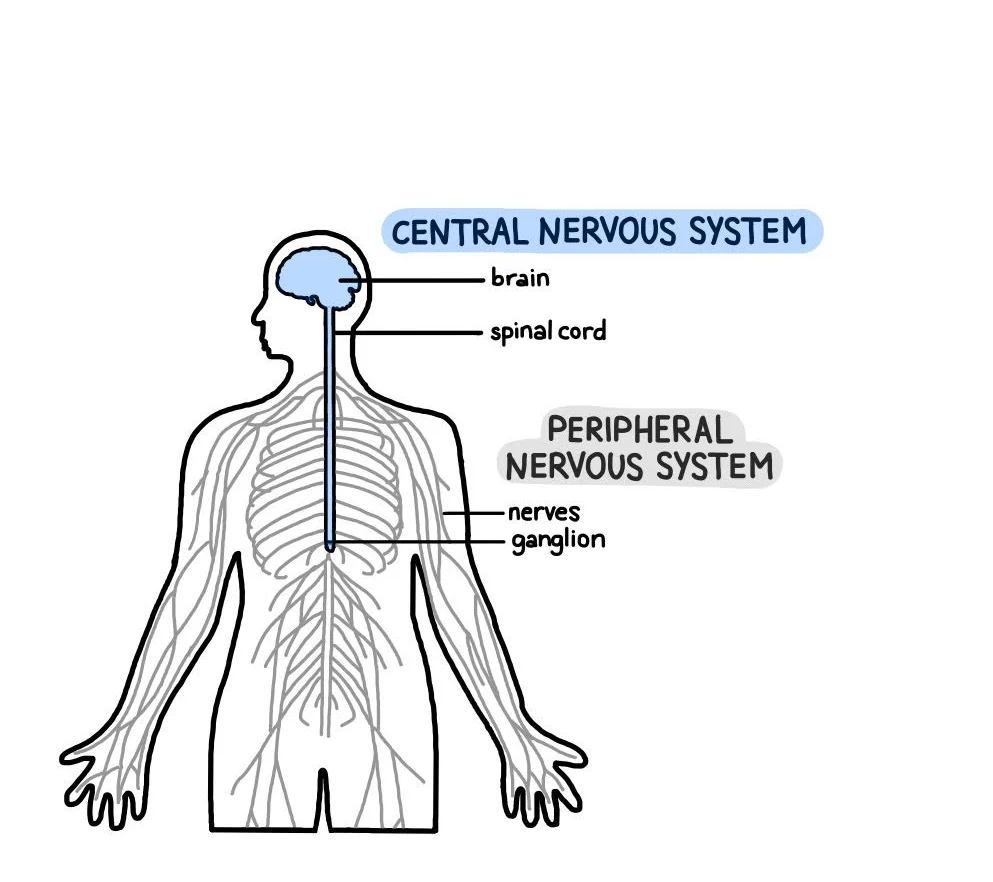
\includegraphics[width=\linewidth,keepaspectratio]{Peripheral_Nervous_System}
		
		{\tiny (Ref: https://www.simplypsychology.org/peripheral-nervous-system.html)}		
		\end{center}	
    \end{column}
  \end{columns}
\end{frame}

%%%%%%%%%%%%%%%%%%%%%%%%%%%%%%%%%%%%%%%%%%%%%%%%%%%%%%%%%%%
\begin{frame}[fragile]\frametitle{Somatic Nervous System (SNS)}
\begin{columns}
    \begin{column}[T]{0.5\linewidth}
      \begin{itemize}
		\item Sensory nerves: Carry impulses to CNS.
		\item Motor nerves: Carry impulses from CNS.
		\item 12 pairs of cranial nerves.
		\item 31 pairs of spinal nerves.
		\item Controls voluntary movements.
	  \end{itemize}
    \end{column}
    \begin{column}[T]{0.5\linewidth}
		\begin{center}
		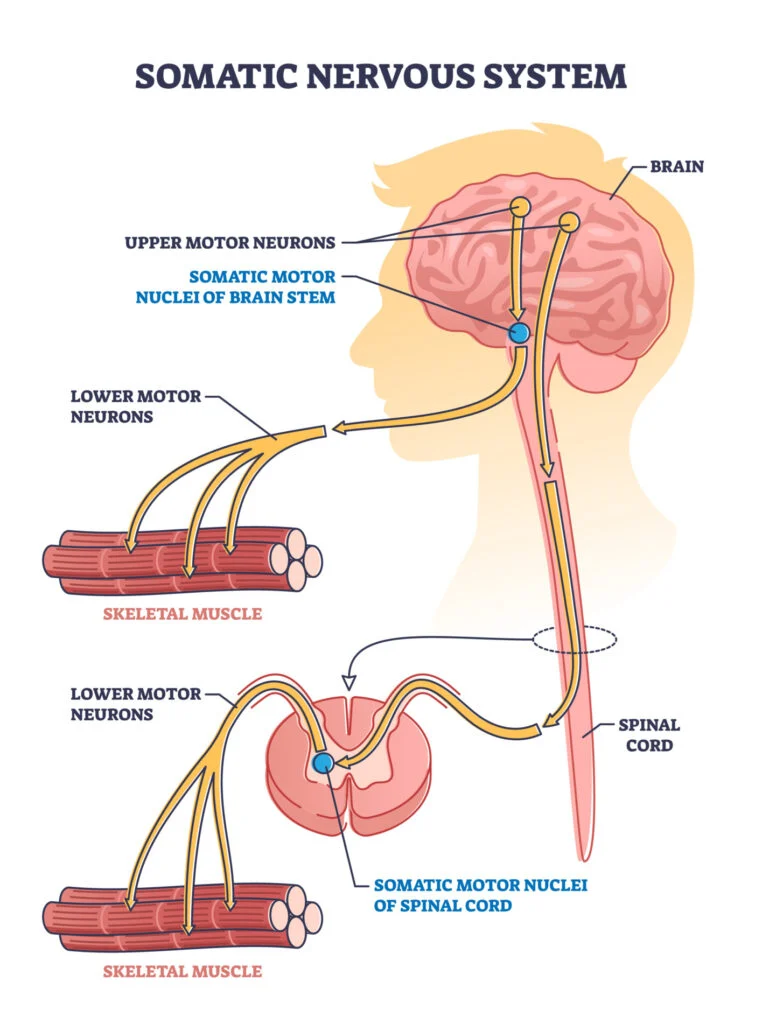
\includegraphics[width=0.8\linewidth,keepaspectratio]{Somatic_nervous_system}
		
		{\tiny (Ref: https://www.simplypsychology.org/somatic-nervous-system.html)}
		\end{center}	
    \end{column}
  \end{columns}
\end{frame}

%%%%%%%%%%%%%%%%%%%%%%%%%%%%%%%%%%%%%%%%%%%%%%%%%%%%%%%%%%%
\begin{frame}[fragile]\frametitle{Autonomic Nervous System (ANS)}
\begin{columns}
    \begin{column}[T]{0.5\linewidth}
      \begin{itemize}
		\item Regulates involuntary actions.
		\item Sympathetic: 'Fight or flight' response.
		\item Parasympathetic: 'Rest and digest' response.
		\item Controls internal organs.
		\item Includes sympathetic and parasympathetic chains.
	  \end{itemize}
    \end{column}
    \begin{column}[T]{0.5\linewidth}
		\begin{center}
		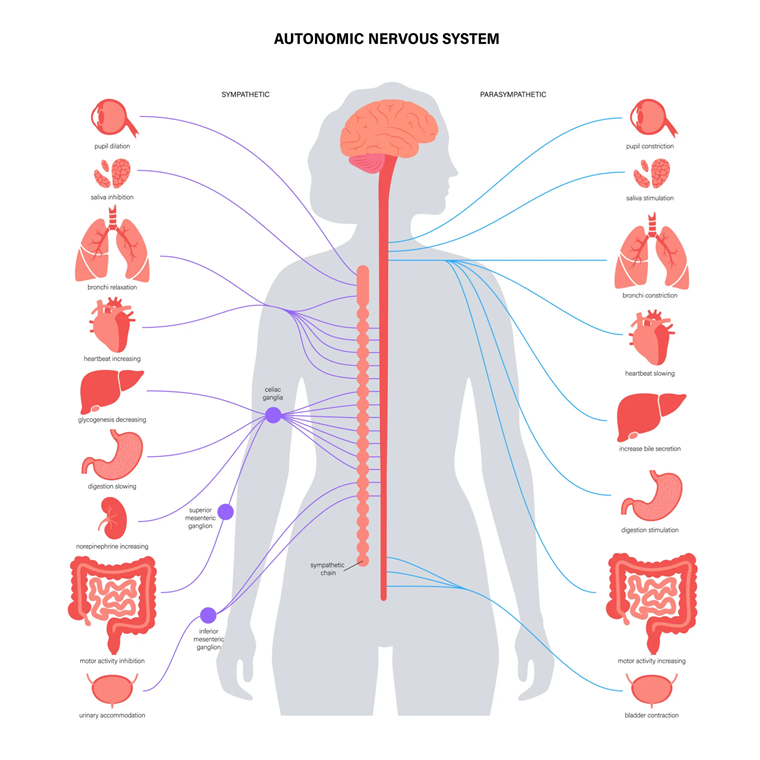
\includegraphics[width=\linewidth,keepaspectratio]{Autonomic_Nervous_System}
		
		{\tiny (Ref: https://www.simplypsychology.org/autonomic-nervous-system.html)}
		\end{center}	
    \end{column}
  \end{columns}
\end{frame}


%%%%%%%%%%%%%%%%%%%%%%%%%%%%%%%%%%%%%%%%%%%%%%%%%%%%%%%%%%%%%%%%%%%%%%%%%%%%%%%%%%
\begin{frame}[fragile]\frametitle{}
\begin{center}
{\Large 3.2  Meaning and Means of health promotion and role of Yoga  in health promotion}
\end{center}
\end{frame}

%%%%%%%%%%%%%%%%%%%%%%%%%%%%%%%%%%%%%%%%%%%%%%%%%%%%%%%%%%%%%%%%%%%%%%%%%%%%%%%%%%
\begin{frame}[fragile]\frametitle{Health Promotion}
    \textbf{Definition of Health:}
    \begin{itemize}
        \item According to the World Health Organization (WHO), health is defined as \textit{“a state of complete physical, mental, and social well-being and not merely the absence of disease or infirmity.”}
    \end{itemize}

    \textbf{Health Promotion:}
    \begin{itemize}
        \item Health promotion involves \textit{encouraging healthy lifestyles} and educating people to increase \textit{awareness} and \textit{well-being}.
        \item Objective: To promote \textit{healthy living} and \textit{prevent disease}.
    \end{itemize}
\end{frame}

%%%%%%%%%%%%%%%%%%%%%%%%%%%%%%%%%%%%%%%%%%%%%%%%%%%%%%%%%%%%%%%%%%%%%%%%%%%%%%%%%%
\begin{frame}[fragile]\frametitle{Role of Yoga in Health Promotion}
    \textbf{Yoga and Health Benefits:}
    \begin{itemize}
        \item Yoga addresses \textit{all aspects of health}:
        \begin{itemize}
            \item \textbf{Cardiovascular Health} - Improves heart function.
            \item \textbf{Muscular Strength and Flexibility} - Enhances physical strength and balance.
            \item \textbf{Stamina and Body Balance} - Builds endurance and stability.
        \end{itemize}
        \item \textbf{Shatkriyas (शट्क्रियास):} Cleanses internal organs.
        \item \textbf{Pranayama (प्राणायाम):} Focuses on breath work for relaxation and increasing \textit{Prana} (प्राण).
        \item \textbf{Dhyana (ध्यान) and Meditation:} Enhances concentration and intuition.
    \end{itemize}

    \textbf{Experiential Learning:}
    \begin{itemize}
        \item Yoga is an \textit{experiential practice}. Regular practice leads to better understanding and control over overall well-being.
        \item Explore different practices like \textbf{Bhakti Yoga (भक्ति योग)}, \textbf{Karma Yoga (कर्म योग)}, and \textbf{Ishvara Pranidhana (ईश्वर प्रणिधान)}, and find what resonates with you.
        \item Stick to the practice as advised by Patanjali (\textit{Abhyasa - अभ्यास}) and observe the effects.
    \end{itemize}
\end{frame}

%%%%%%%%%%%%%%%%%%%%%%%%%%%%%%%%%%%%%%%%%%%%%%%%%%%%%%%%%%%
\begin{frame}[fragile]\frametitle{Effects of Hatha Yoga Practices}
      \begin{itemize}
        \item Enhances flexibility in tendons, muscles, and spine.
        \item Improves overall blood flow and oxygen delivery.
        \item Supports cardiovascular health and lowers blood pressure.
        \item Facilitates lymphatic system function and detoxification.
        \item Corrects poor posture and improves body alignment.
        \item Relieves pain and tension in joints and muscles.
        \item Loosens tight areas like neck and shoulders.
        \item Promotes mental well-being alongside physical health.
      \end{itemize}
\end{frame}

%%%%%%%%%%%%%%%%%%%%%%%%%%%%%%%%%%%%%%%%%%%%%%%%%%%%%%%%%%%
\begin{frame}[fragile]\frametitle{Limitations and Contraindications of Yoga Practices}
      \begin{itemize}
        \item Awareness of contraindications is essential before starting practice.
        \item Yoga is preventive, not primarily curative; used as an alternative therapy.
        \item Individual differences mean not all practices suit everyone; avoid comparison.
        \item More effective for functional disorders than for organic conditions.
        \item Not a cure for conditions like cancer; helps in managing symptoms and improving strength.
        \item Not a standalone remedy for issues like obesity; requires diet and lifestyle changes.
        \item Best used as a complementary therapy alongside conventional treatments.
      \end{itemize}
\end{frame}


%%%%%%%%%%%%%%%%%%%%%%%%%%%%%%%%%%%%%%%%%%%%%%%%%%%%%%%%%%%%%%%%%%%%%%%%%%%%%%%%%%
\begin{frame}[fragile]\frametitle{}
\begin{center}
{\Large 3.3 Yogic positive Attitudes}
\end{center}
\end{frame}

%%%%%%%%%%%%%%%%%%%%%%%%%%%%%%%%%%%%%%%%%%%%%%%%%%%%%%%%%%%
\begin{frame}[fragile]\frametitle{Yogic Positive Attitudes in Yogasutra: Chitta Prasadana}

मैत्रीकरुणामुदितोपेक्षाणां सुखदुःखपुण्यापुण्यिवषयाणां भावनातिश्चत्तप्रसादनम् ॥   १ . ३३॥

      \begin{itemize}
        \item \textbf{Maitri:} Cultivating friendship and kindness towards others.
        \item \textbf{Karuna:} Practicing compassion and empathy for those in suffering.
        \item \textbf{Mudita:} Experiencing joy and appreciation for others' happiness.
        \item \textbf{Upeksha:} Maintaining equanimity and detachment from the fluctuations of life.
        \item \textbf{Mind Purification:} Cleansing the mind of negative emotions and thoughts.
        \item \textbf{Inner Peace:} Creating a serene mental environment through positive attitudes.
        \item \textbf{Emotional Balance:} Developing stability in emotional responses.
        \item \textbf{Self-Improvement:} Enhancing personal growth through these attitudes.
        \item \textbf{Harmonious Relationships:} Fostering better interactions with others.
        \item \textbf{Mindful Awareness:} Increasing mindfulness and self-awareness in daily life.
      \end{itemize}

\end{frame}

%%%%%%%%%%%%%%%%%%%%%%%%%%%%%%%%%%%%%%%%%%%%%%%%%%%%%%%%%%%%%%%%%%%%%%%%%%%%%%%%%%
\begin{frame}[fragile]\frametitle{}
\begin{center}
{\Large 3.4 Concept of Bhavas}
\end{center}
\end{frame}

% %%%%%%%%%%%%%%%%%%%%%%%%%%%%%%%%%%%%%%%%%%%%%%%%%%%%%%%%%%%
% \begin{frame}[fragile]\frametitle{Concept of Bhavas}

      % \begin{itemize}
        % \item Bhavas are essential attitudes for mental and emotional well-being.
        % \item They include Dharma, Jnana, Vairagya, and Aishwarya.
        % \item Each Bhava contributes uniquely to balanced living and personal growth.
      % \end{itemize}

% \end{frame}

% %%%%%%%%%%%%%%%%%%%%%%%%%%%%%%%%%%%%%%%%%%%%%%%%%%%%%%%%%%%
% \begin{frame}[fragile]\frametitle{Dharma (Duty)}

      % \begin{itemize}
        % \item \textbf{Sanskrit Verse:} 
        
        % योगिश्चत्तवृित्तिनरोधः   ॥   १ . २॥ \\
        % Yogachittavrittinirodhah || 1.2
        
        % \item Dharma is the highest duty to maintain a balanced mind.
        % \item It involves using Yoga techniques like Asana, Pranayama, and Meditation.
        % \item Aim to keep a positive state even amidst life’s ups and downs.

        % \item \textbf{Sanskrit Verse:} 
        
        % दृग्दशर्नशक्त्योरेकात्मतेवािस्मता   ॥   २ . ६॥ \\
        % Drk-Daesanasaktyoh-Ekatmate-Iva-Asmita || 2.6
        
        % \item Gain understanding and knowledge before taking action.
        % \item Learn from self-experience; view learning as personal growth.
        % \item Avoid ego by recognizing that knowledge is personal and subjective.
      % \end{itemize}	  

% \end{frame}

% %%%%%%%%%%%%%%%%%%%%%%%%%%%%%%%%%%%%%%%%%%%%%%%%%%%%%%%%%%%
% \begin{frame}[fragile]\frametitle{Vairagya (Objectivity) and Aishwarya (Self-Reliance)}

      % \begin{itemize}
        % \item \textbf{Vairagya (Objectivity):}
        
        % तत्परं   पुरुषख्यातेगुर्णवैतृष्ण्यम्   ॥   १ . १६॥ \\
        % Tatparam Purusakhyateh Gunavaitrshnyam || 1.16
        
        % \item Cultivate detachment and a witness-like attitude.
        % \item Surrender ego and remain objective in life.
        % \item \textbf{Aishwarya (Self-Reliance):}
        
        % तत्र   स्थितौ   यत्नोऽभ्यासः   ॥   १ . १३॥ \\
        % Tatra sthitau-yatnah abhyasah || 1.13
        
        % \item Achieve self-reliance and perfection through consistent practice.
        % \item Increases willpower, confidence, and joy.
      % \end{itemize}

% \end{frame}

%%%%%%%%%%%%%%%%%%%%%%%%%%%%%%%%%%%%%%%%%%%%%%%%%%%%%%%%%%%%%%%%%%%%%%%%%%%%%%%%%%
\begin{frame}[fragile]\frametitle{Concept of Bhava}
    \textbf{Bhava (भाव)} can be understood as:
    \begin{itemize}
        \item A certain \textbf{state of mind}
        \item A \textbf{feeling}, \textbf{emotion}, or \textbf{attitude}
    \end{itemize}

    \textbf{Yogic Science:}
    \begin{itemize}
        \item Yogic processes work on the mind by generating specific \textit{Bhava} within oneself.
        \item Examples: Forward bending postures and chest openers.
    \end{itemize}
    
    \textbf{Types of Bhava:}
    \begin{itemize}
        \item \textbf{Positive Bhavas:} Dharma Bhava (धर्म भाव), Jnana Bhava (ज्ञान भाव), Vairagya Bhava (वैराग्य भाव), and Aishwarya Bhava (ऐश्वर्य भाव)
        \item \textbf{Negative Bhavas:} Adharma Bhava (अधर्म भाव), Raga Bhava (राग भाव), Dvesha Bhava (द्वेष भाव), and Ajnana Bhava (अज्ञान भाव)
    \end{itemize}
\end{frame}


%%%%%%%%%%%%%%%%%%%%%%%%%%%%%%%%%%%%%%%%%%%%%%%%%%%%%%%%%%%%%%%%%%%%%%%%%%%%%%%%%%
\begin{frame}[fragile]\frametitle{Understanding and Practicing Bhava}
    \textbf{Negative Bhavas:}
    \begin{itemize}
        \item \textbf{Adharma Bhava (अधर्म भाव)} - Unrighteousness
        \item \textbf{Raga Bhava (राग भाव)} - Attachment
        \item \textbf{Dvesha Bhava (द्वेष भाव)} - Aversion
        \item \textbf{Ajnana Bhava (अज्ञान भाव)} - Ignorance
    \end{itemize}
    
    \textbf{Positive Bhavas:}
    \begin{itemize}
        \item \textbf{Dharma Bhava (धर्म भाव)} - Discipline and Duty
        \item \textbf{Jnana Bhava (ज्ञान भाव)} - Knowledge and Clarity
        \item \textbf{Vairagya Bhava (वैराग्य भाव)} - Detachment and Letting Go
        \item \textbf{Aishwarya Bhava (ऐश्वर्य भाव)} - Strength and Power
    \end{itemize}
    
    \textbf{Practices to Enhance Positive Bhavas:}
    \begin{itemize}
        \item \textbf{Dharma Bhava:} Practices like Padmasana (पद्मासन), Sukhasana (सुखासन), and Yamas (यम) and Niyamas (नियम).
        \item \textbf{Jnana Bhava:} Balancing postures and practices like Kapalabhati (कपालभाति) and Trataka (त्राटक).
        \item \textbf{Vairagya Bhava:} Forward bending postures.
        \item \textbf{Aishwarya Bhava:} Strengthening self-awareness and introspection.
    \end{itemize}
\end{frame}


%%%%%%%%%%%%%%%%%%%%%%%%%%%%%%%%%%%%%%%%%%%%%%%%%%%%%%%%%%%%%%%%%%%%%%%%%%%%%%%%%%
\begin{frame}[fragile]\frametitle{}
\begin{center}
{\Large 3.5 Dincharya and Ritucharya with respect to Yogic lifestyle}
\end{center}
\end{frame}

% %%%%%%%%%%%%%%%%%%%%%%%%%%%%%%%%%%%%%%%%%%%%%%%%%%%%%%%%%%%%%%%%%%%%%%%%%%%%%%%%%%
% \begin{frame}[fragile]\frametitle{Ayurvedic Principles: Dinacharya and Ritucharya}

      % \begin{itemize}
        % \item \textbf{Relative Health Concepts:} What is healthy or unhealthy depends on individual factors like age, constitution, and health conditions.
        % \item \textbf{Context Matters:} Diet and lifestyle recommendations vary based on factors such as season, disease state, and geographical location.
        % \item \textbf{Dinacharya (Daily Regimen):} Ayurveda prescribes daily routines to balance Doshas and prevent disorders.
        % \item \textbf{Ritucharya (Seasonal Regimen):} Seasonal guidelines help align lifestyle with environmental changes to maintain health.
        % \item \textbf{Preventive Focus:} Ayurveda emphasizes prevention over cure; following Dinacharya and Ritucharya enhances immunity and life quality.
        % \item \textbf{Long-Term Benefits:} Adhering to these regimens reduces risk of future disorders and improves overall life expectancy.
        % \item \textbf{Scientific Basis:} Ancient Ayurvedic principles, tested over centuries, remain relevant and beneficial globally.
        % \item \textbf{Universal Relevance:} Basic Ayurvedic principles apply across different climates and regions, adapting tools but maintaining core concepts.
      % \end{itemize}

% \end{frame}

% %%%%%%%%%%%%%%%%%%%%%%%%%%%%%%%%%%%%%%%%%%%%%%%%%%%%%%%%%%%%%%%%%%%%%%%%%%%%%%%%%%
% \begin{frame}[fragile]\frametitle{Ritucharya: Seasonal Regimen}

      % \begin{itemize}
        % \item \textbf{Similarity-Dissimilarity Doctrine:} 
        
        % “A similar material enriches the similar in the body, while a dissimilar material depletes its counterpart.”
        
        % \item \textbf{Seasonal Impact on Doshas:} 
        % \begin{itemize}
            % \item Cold weather increases Vata Dosha and decreases Pitta Dosha.
            % \item Dry conditions can aggravate Kapha Dosha.
        % \end{itemize}
        % \item \textbf{Balancing External Influences:} 
        % \begin{itemize}
            % \item Ritucharya helps balance the internal environment against seasonal changes.
            % \item Lifestyle and diet are adapted to minimize adverse effects.
        % \end{itemize}
        % \item \textbf{Dosha Reactions:} 
        % \begin{itemize}
            % \item \textbf{Sanchaya:} Accumulation of Dosha.
            % \item \textbf{Prakopa:} Aggravation of Dosha.
            % \item \textbf{Prashama:} Pacification of Dosha.
        % \end{itemize}
        % \item \textbf{Maintaining Dosha Equilibrium:} 
        % \begin{itemize}
            % \item Aim to achieve Dosha-Samya (Dosha equilibrium).
            % \item Focus on transitional periods (Ritusandhi) between seasons to prevent diseases.
        % \end{itemize}
        % \item \textbf{Health Benefits:} 
        % \begin{itemize}
            % \item Enhances immunity, prevents seasonal diseases, and improves quality of life.
        % \end{itemize}
      % \end{itemize}

% \end{frame}

% %%%%%%%%%%%%%%%%%%%%%%%%%%%%%%%%%%%%%%%%%%%%%%%%%%%%%%%%%%%%%%%%%%%%%%%%%%%%%%%%%%
% \begin{frame}[fragile]\frametitle{Ritusandhi: Transitional Period Between Seasons}

      % \begin{itemize}
        % \item \textbf{Definition:} 
        
        % Ritusandhi refers to the transitional period between two seasons, lasting about two weeks.
        
        % \item \textbf{Duration:} 
        % \begin{itemize}
            % \item First week: Last seven days of the current season.
            % \item Second week: First seven days of the upcoming season.
        % \end{itemize}
        % \item \textbf{Gradual Changes:} 
        % \begin{itemize}
            % \item Seasonal transitions are gradual, not abrupt.
            % \item Adjustments in diet and routine should be made gradually.
        % \end{itemize}
        % \item \textbf{Caution Required:} 
        % \begin{itemize}
            % \item This period is delicate; careful management of diet and routine is crucial.
            % \item Avoid practices that disrupt Dosha balance.
        % \end{itemize}
        % \item \textbf{Health Risks:} 
        % \begin{itemize}
            % \item Common health issues during Ritusandhi include colds, flu, and fever.
            % \item Hospitals often see increased admissions during this time.
        % \end{itemize}
        % \item \textbf{Preventive Measures:} 
        % \begin{itemize}
            % \item Adhere to Ayurvedic recommendations to maintain health and prevent illness.
        % \end{itemize}
      % \end{itemize}

% \end{frame}

% %%%%%%%%%%%%%%%%%%%%%%%%%%%%%%%%%%%%%%%%%%%%%%%%%%%%%%%%%%%%%%%%%%%%%%%%%%%%%%%%%%
% \begin{frame}[fragile]\frametitle{Classification of Seasons}

      % \begin{itemize}
        % \item \textbf{Samwatsara (Year):} 
        
        % A year consists of two Ayanas and six Ritus.
        
        % \item \textbf{Ayanas (Semesters):} 
        % \begin{itemize}
            % \item \textbf{Uttarayana (Northern Solstice):}
            
            % The Sun moves northward, taking moisture from the earth (Adanakala).
            
            % \item \textbf{Dakshinayana (Southern Solstice):}
            
            % The Sun moves southward, giving moisture to the earth (Visargakala).
            
        % \end{itemize}
        % \item \textbf{Uttarayana Seasons:}
        % \begin{itemize}
            % \item \textbf{Shishira:} Late winter.
            % \item \textbf{Vasanta:} Spring.
            % \item \textbf{Grishma:} Summer.
        % \end{itemize}
        % \item \textbf{Dakshinayana Seasons:}
        % \begin{itemize}
            % \item \textbf{Varsha:} Rainy season.
            % \item \textbf{Sharad:} Autumn.
            % \item \textbf{Hemanta:} Early winter.
        % \end{itemize}
        % \item \textbf{Seasonal Attributes:} 
        % \begin{itemize}
            % \item Understanding seasonal attributes helps in selecting suitable food and activities.
        % \end{itemize}
      % \end{itemize}

% \end{frame}

% %%%%%%%%%%%%%%%%%%%%%%%%%%%%%%%%%%%%%%%%%%%%%%%%%%%%%%%%%%%%%%%%%%%%%%%%%%%%%%%%%%
% \begin{frame}[fragile]\frametitle{Dinacharya: Daily Regimen}

      % \begin{itemize}
        % \item \textbf{Concept:} 
        
        % A day reflects seasonal and yearly attributes, guiding daily health practices.
        
        % \item \textbf{Purpose:} 
        % \begin{itemize}
            % \item Promotes long-term health and well-being.
        % \end{itemize}
        % \item \textbf{Daily Routine Includes:}
        % \begin{itemize}
            % \item \textbf{Morning:} Wake up, elimination, oral care, self-massage.
            % \item \textbf{Day:} Exercise, bathing, diet, social etiquette.
            % \item \textbf{Evening:} Relaxation, bedtime routine, sexual health.
        % \end{itemize}
        % \item \textbf{Guidance:} 
        % \begin{itemize}
            % \item Detailed Ayurveda instructions on practices and materials.
        % \end{itemize}
      % \end{itemize}

% \end{frame}

% %%%%%%%%%%%%%%%%%%%%%%%%%%%%%%%%%%%%%%%%%%%%%%%%%%%%%%%%%%%%%%%%%%%%%%%%%%%%%%%%%%
% \begin{frame}[fragile]\frametitle{Ayurvedic Dinacharya: Daily Cycles and Practices}

      % \begin{itemize}
        % \item \textbf{Daily Cycles:}
        % \begin{itemize}
            % \item \textbf{Sun Cycle (6:00 AM - 6:00 PM):}
            % \begin{itemize}
                % \item 6:00 AM - 10:00 AM: Kapha
                % \item 10:00 AM - 2:00 PM: Pitta
                % \item 2:00 PM - 6:00 PM: Vata
            % \end{itemize}
            % \item \textbf{Moon Cycle (6:00 PM - 6:00 AM):}
            % \begin{itemize}
                % \item 6:00 PM - 10:00 PM: Kapha
                % \item 10:00 PM - 2:00 AM: Pitta
                % \item 2:00 AM - 6:00 AM: Vata
            % \end{itemize}
        % \end{itemize}
        % \item \textbf{Recommended Practices:}
        % \begin{itemize}
            % \item Wake up, elimination, face wash, brushing teeth, tongue cleaning.
            % \item Gargle, nasal cleaning, massage, exercise, herbal scrub, bathing.
            % \item Worship, clothing \& shoes, work, sleep \& sex.
        % \end{itemize}
        % \item \textbf{Benefits:} 
        % \begin{itemize}
            % \item Connects with nature, prevents diseases, reduces stress.
            % \item Enhances digestion, promotes discipline, peace, happiness, and longevity.
        % \end{itemize}
      % \end{itemize}

% \end{frame}


%%%%%%%%%%%%%%%%%%%%%%%%%%%%%%%%%%%%%%%%%%%%%%%%%%%%%%%%%%%%%%%%%%%%%%%%%%%%%%%%%%
\begin{frame}[fragile]\frametitle{Dinacharya and Ritucharya}
    \textbf{Dinacharya (दिनचर्या)}: Daily Routine
    \begin{itemize}
        \item Refers to daily activities and routines.
        \item Helps in maintaining daily health and balance.
        \item Based on Ayurvedic principles and body doshas.
    \end{itemize}

    \textbf{Ritucharya (ऋतुचर्या )}: Seasonal Routine
    \begin{itemize}
        \item Refers to seasonal activities and diet.
        \item Aims at promoting health according to seasonal changes.
        \item Adjusts diet and activities based on the season.
    \end{itemize}

    \textbf{दोष  Doshas and Daily Phases:}
    \begin{itemize}
        \item \textbf{Vata (वात)}: 2:00 AM - 6:00 AM, 2:00 PM - 6:00 PM
        \item \textbf{Kapha (कफ)}: 6:00 AM - 10:00 AM, 6:00 PM - 10:00 PM
        \item \textbf{Pitta (पित्त)}: 10:00 AM - 2:00 PM, 10:00 PM - 2:00 AM
    \end{itemize}
\end{frame}

%%%%%%%%%%%%%%%%%%%%%%%%%%%%%%%%%%%%%%%%%%%%%%%%%%%%%%%%%%%%%%%%%%%%%%%%%%%%%%%%%%
\begin{frame}[fragile]\frametitle{Daily Guidelines (Dinacharya)}
    \textbf{Suggested Routine:}
    \begin{itemize}
        \item \textbf{Brahmamuhurta (ब्राह्ममुहूर्त)}: Wake up 1-1.5 hours before sunrise.
        \item \textbf{Morning Routine:}
        \begin{itemize}
            \item Mouthwash (कंठधावन)
            \item Toothbrush (दन्तधावन)
            \item Tongue cleaning (जिव्हा-धावन)
            \item Oil pulling (कौण्डल्या)
            \item Face wash (अर्घ्यम्)
        \end{itemize}
        \item \textbf{Daily Activities:}
        \begin{itemize}
            \item Physical exercise (व्यायाम)
            \item Body massage (अभ्यंग)
            \item Bathing (स्नान)
            \item Dressing and grooming (वस्त्रादि)
        \end{itemize}
    \end{itemize}
\end{frame}

%%%%%%%%%%%%%%%%%%%%%%%%%%%%%%%%%%%%%%%%%%%%%%%%%%%%%%%%%%%%%%%%%%%%%%%%%%%%%%%%%%
\begin{frame}[fragile]\frametitle{Seasonal Guidelines (Ritucharya)}
    \textbf{Seasons and Doshas:}
    \begin{itemize}
        \item \textbf{Adana Kal (आदन काल)}: 
        \begin{itemize}
            \item Shishira (शिशिर) - Winter
            \item Vasant (वसंत) - Spring
            \item Grishma (ग्रीष्म) - Summer
        \end{itemize}
        \item \textbf{Visarga Kal (विसर्ग काल)}:
        \begin{itemize}
            \item Varsha (वर्षा) - Monsoon
            \item Sharad (शरद्) - Autumn
            \item Hemanta (हेमन्त) - Late Autumn/Pre-Winter
        \end{itemize}
    \end{itemize}

    \textbf{Guidelines:}
    \begin{itemize}
        \item Adjust diet and activities according to the season.
        \item Consult an Ayurvedic practitioner for personalized routines.
    \end{itemize}
\end{frame}

%%%%%%%%%%%%%%%%%%%%%%%%%%%%%%%%%%%%%%%%%%%%%%%%%%%%%%%%%%%%%%%%%%%%%%%%%%%%%%%%%%
\begin{frame}[fragile]\frametitle{}
\begin{center}
{\Large 3.6 Holistic approach of Yoga towards health and Diseases}
\end{center}
\end{frame}

% %%%%%%%%%%%%%%%%%%%%%%%%%%%%%%%%%%%%%%%%%%%%%%%%%%%%%%%%%%%%%%%%%%%%%%%%%%%%%%%%%%
% \begin{frame}[fragile]\frametitle{Yoga, Health, and Awareness}

      % \begin{itemize}
        % \item \textbf{Mindset and Health:} 
        
        % "Man today is sick because he thinks he is sick. Sickness and disease have no place in a person who does not accept self-laments." 
        
        % \item \textbf{Swami Satyananda Saraswati's View:}
        % \begin{itemize}
            % \item Disease is not fate but a call for change and growth.
            % \item Yoga helps break the illusion of disease as inescapable.
        % \end{itemize}
        % \item \textbf{Yoga's Role:}
        % \begin{itemize}
            % \item Yoga and medicine complement each other in restoring health.
            % \item Yoga views disease as a teacher and guide to balance.
        % \end{itemize}
        % \item \textbf{Disease as a Teacher:}
        % \begin{itemize}
            % \item Indicates lifestyle or mental errors.
            % \item Signals the need for lifestyle changes for better health and joy.
        % \end{itemize}
      % \end{itemize}

% \end{frame}

% %%%%%%%%%%%%%%%%%%%%%%%%%%%%%%%%%%%%%%%%%%%%%%%%%%%%%%%%%%%%%%%%%%%%%%%%%%%%%%%%%%
% \begin{frame}[fragile]\frametitle{Holistic Health and the Yogic Approach}

      % \begin{itemize}
        % \item \textbf{Regaining Awareness:}
        % \begin{itemize}
            % \item Disease forces awareness of natural law transgressions.
            % \item Yogic practices restore balance and understanding.
        % \end{itemize}
        % \item \textbf{WHO Definition of Health:}
        
        % Health is physical, mental, intellectual, and spiritual well-being—not just a disease-free body.
        
        % \item \textbf{Holistic Treatment Approach:}
        % \begin{itemize}
            % \item Traditional Yoga, therapeutic Yoga, and Ayurveda address root causes of diseases.
            % \item A holistic, empathetic approach is essential in yoga practice.
        % \end{itemize}
        % \item \textbf{Yoga Teacher's Role:}
        % \begin{itemize}
            % \item Provide complete solutions with empathy for physical and mental complaints.
        % \end{itemize}
      % \end{itemize}

% \end{frame}


%%%%%%%%%%%%%%%%%%%%%%%%%%%%%%%%%%%%%%%%%%%%%%%%%%%%%%%%%%%%%%%%%%%%%%%%%%%%%%%%%%
\begin{frame}[fragile]\frametitle{Holistic Approach of Yoga Towards Health}
    \textbf{Yoga and Health:}
    \begin{itemize}
        \item Yoga practices have gained global recognition for maintaining overall health.
        \item Unlike medicine, which treats illness after it occurs, yoga aims to prevent illness before it begins.
        \item \textbf{Patanjali's Insight:} \textit{दुःखमअनात्म} (Dukham Anātma) – To avoid suffering that has not yet occurred.
    \end{itemize}

    \textbf{Prevention Aspect:}
    \begin{itemize}
        \item Yoga practices help in preventing diseases and maintaining overall health.
        \item Regular practice is associated with reduced risk of illness and enhanced well-being.
    \end{itemize}
\end{frame}


%%%%%%%%%%%%%%%%%%%%%%%%%%%%%%%%%%%%%%%%%%%%%%%%%%%%%%%%%%%%%%%%%%%%%%%%%%%%%%%%%%
\begin{frame}[fragile]\frametitle{Yoga in Disease Management and Therapy}
    \textbf{Yoga as Therapy:}
    \begin{itemize}
        \item Yoga is also effective in managing existing illnesses.
        \item During the COVID-19 pandemic, practices like pranayama and breathwork were recommended to increase lung capacity and oxygen levels.
        \item Research on kriyas like \textit{कपालभाति} (Kapalbhati) and \textit{सूर्यनमस्कार} (Suryanamaskar) showed benefits in lung diffusion capacity and oxygen levels.
    \end{itemize}

    \textbf{Holistic Benefits:}
    \begin{itemize}
        \item Yoga addresses physical, mental, social, and spiritual well-being.
        \item Practices are designed to enhance overall health and manage stress, leading to a balanced life.
    \end{itemize}
\end{frame}

%%%%%%%%%%%%%%%%%%%%%%%%%%%%%%%%%%%%%%%%%%%%%%%%%%%%%%%%%%%%%%%%%%%%%%%%%%%%%%%%%%
\begin{frame}[fragile]\frametitle{}
\begin{center}
{\Large 3.7 Introduction to first aid and Cardio Pulmonary Resuscitation (CPR)}
\end{center}
\end{frame}

%%%%%%%%%%%%%%%%%%%%%%%%%%%%%%%%%%%%%%%%%%%%%%%%%%%%%%%%%%%%%%%%%%%%%%%%%%%%%%%%%%
\begin{frame}[fragile]\frametitle{Introduction to First Aid}
    \textbf{What is First Aid?}
    \begin{itemize}
        \item Immediate medical attention provided in case of injury.
        \item Includes actions like applying bandages, cleaning minor cuts and scratches, and providing fluids to restore hydration.
    \end{itemize}
\end{frame}


%%%%%%%%%%%%%%%%%%%%%%%%%%%%%%%%%%%%%%%%%%%%%%%%%%%%%%%%%%%%%%%%%%%%%%%%%%%%%%%%%%
\begin{frame}[fragile]\frametitle{Introduction to First Aid}

      \begin{itemize}
        \item \textbf{Definition:} 
        
        Immediate care given to an injured or ill person until professional help arrives.
        
        \item \textbf{First Aid Kit Essentials:} 
        \begin{itemize}
            \item Adhesive bandages, gauze pads, antiseptic wipes.
            \item Scissors, tweezers, adhesive tape.
            \item Pain relievers, burn cream, digital thermometer.
        \end{itemize}
        \item \textbf{Basic First Aid Procedures:} 
        \begin{itemize}
            \item \textbf{Wounds:} Clean with water, apply antiseptic, and bandage.
            \item \textbf{Burns:} Cool with running water, cover with a clean cloth.
            \item \textbf{Fractures:} Immobilize the area, seek medical help.
        \end{itemize}
        \item \textbf{Importance of Training:} 
        
        Effective response in emergencies and potential life-saving.
        
      \end{itemize}

\end{frame}

%%%%%%%%%%%%%%%%%%%%%%%%%%%%%%%%%%%%%%%%%%%%%%%%%%%%%%%%%%%%%%%%%%%%%%%%%%%%%%%%%%
\begin{frame}[fragile]\frametitle{Introduction to CPR}
    \textbf{What is CPR?}
    \begin{itemize}
        \item Cardiopulmonary Resuscitation (CPR) is a life-saving procedure performed when the heart stops beating.
        \item CPR can double or triple the chances of survival after cardiac arrest.
        \item \textbf{Types of CPR:}
        \begin{itemize}
            \item \textbf{Trained Professionals:} Combination of 30 compressions and 2 breaths.
            \item \textbf{Untrained Individuals:} Compression-only CPR.
        \end{itemize}
    \end{itemize}
\end{frame}

%%%%%%%%%%%%%%%%%%%%%%%%%%%%%%%%%%%%%%%%%%%%%%%%%%%%%%%%%%%%%%%%%%%%%%%%%%%%%%%%%%
\begin{frame}[fragile]\frametitle{Importance of CPR Training}
    \textbf{CPR Certification:}
    \begin{itemize}
        \item In India, CPR certification is not mandatory for yoga teachers.
        \item In Western countries, it might be required by some studios.
        \item CPR training is beneficial for everyone and can be obtained from various agencies and hospitals.
    \end{itemize}
    
    \textbf{Action Items:}
    \begin{itemize}
        \item Watch the reference video provided by the Global Association of Indian Medical Students.
        \item Consider obtaining CPR certification to enhance your skills and knowledge.
    \end{itemize}
\end{frame}


%%%%%%%%%%%%%%%%%%%%%%%%%%%%%%%%%%%%%%%%%%%%%%%%%%%%%%%%%%%%%%%%%%%%%%%%%%%%%%%%%%
\begin{frame}[fragile]\frametitle{Introduction to CPR (Cardio Pulmonary Resuscitation)}

      \begin{itemize}
        \item \textbf{Definition:} 
        
        A life-saving technique used when someone’s heartbeat or breathing has stopped.
        
        \item \textbf{CPR Steps:} 
        \begin{itemize}
            \item \textbf{Check Response:} Shake and shout to see if the person responds.
            \item \textbf{Call for Help:} Dial emergency services if no response.
            \item \textbf{Chest Compression:} Push hard and fast (100-120 compression per minute).
            \item \textbf{Rescue Breaths:} If trained, give 2 breaths after every 30 compression.
        \end{itemize}
        \item \textbf{Compression Depth and Rate:} 
        \begin{itemize}
            \item Depth: At least 2 inches (5 cm).
            \item Rate: 100-120 compression per minute.
        \end{itemize}
        \item \textbf{When to Perform CPR:} 
        
        When the person is unresponsive and not breathing normally.
        
      \end{itemize}

\end{frame}

%%%%%%%%%%%%%%%%%%%%%%%%%%%%%%%%%%%%%%%%%%%%%%%%%%%%%%%%%%%%%%%%%%%%%%%%%%%%%%%%%%
\begin{frame}[fragile]\frametitle{}
\begin{center}
{\Large 3.8 Yogic Management of stress and its consequences}
\end{center}
\end{frame}

%%%%%%%%%%%%%%%%%%%%%%%%%%%%%%%%%%%%%%%%%%%%%%%%%%%%%%%%%%%%%%%%%%%%%%%%%%%%%%%%%%
\begin{frame}[fragile]\frametitle{Human Psyche: Modern and Yogic Concepts}

      \begin{itemize}
        \item \textbf{Psychology:}
        
        The scientific study of mental processes and behavior, impacting various life spheres including family, education, and health.
        
        \item \textbf{Behavior:}
        \begin{itemize}
            \item \textbf{Overt Behavior:} Visible actions or reactions to external stimuli.
            \item \textbf{Covert Behavior:} Internal mental processes and phenomena.
        \end{itemize}
        \item \textbf{Consciousness:}
        
        A non-physical, self-directed entity responsible for creating, retaining, and annihilating concepts of Self and Universe.
        
        \item \textbf{Consciousness Expansion:}
        \begin{itemize}
            \item Yogic techniques help expand awareness and unite Atman (Self) with Paramatman (Supreme Self).
        \end{itemize}
      \end{itemize}

\end{frame}

%%%%%%%%%%%%%%%%%%%%%%%%%%%%%%%%%%%%%%%%%%%%%%%%%%%%%%%%%%%%%%%%%%%%%%%%%%%%%%%%%%
\begin{frame}[fragile]\frametitle{Indian Model of Personality}

      \begin{itemize}
        \item \textbf{Upanishadic Personality Model:}
        
        Described through 5 energy sheaths or \textit{Koshas} (\textit{कोश}).
        
        \item \textbf{Annamaya Kosha:} 
        
        Food sheath nourished by \textit{Anna} (\textit{अन्न} - food).
        
        \item \textbf{Pranamaya Kosha:}
        
        Vital air sheath nourished by \textit{Prana} (\textit{प्राण} - bio-energy).
        
        \item \textbf{Manomaya Kosha:}
        
        Mental sheath nourished by \textit{Pratyahara} (\textit{प्रत्याहार} - withdrawal of senses).
        
        \item \textbf{Vijnyanmaya Kosha:}
        
        Intellectual sheath nourished by \textit{Dhyana} (\textit{ध्यान} - meditation).
        
        \item \textbf{Anandamaya Kosha:}
        
        Bliss sheath nourished by \textit{Samadhi} (\textit{समाधि} - state of bliss).
        
      \end{itemize}

\end{frame}


%%%%%%%%%%%%%%%%%%%%%%%%%%%%%%%%%%%%%%%%%%%%%%%%%%%%%%%%%%%%%%%%%%%%%%%%%%%%%%%%%%
\begin{frame}[fragile]\frametitle{Development of Consciousness: The Three Gunas}

      \begin{itemize}
        \item \textbf{Three Gunas:}
        
        Fundamental qualities influencing consciousness and behavior.
        
        \item \textbf{Sattva} (\textit{सत्त्व}): Stability
        \begin{itemize}
            \item Attributes: Love, compassion, honesty, and calm.
        \end{itemize}
        \item \textbf{Rajas} (\textit{रजस्}): Activation
        \begin{itemize}
            \item Attributes: Action, ambition, desire, and leadership.
        \end{itemize}
        \item \textbf{Tamas} (\textit{तमस्}): Inertia
        \begin{itemize}
            \item Attributes: Laziness, sleep, indolence, and aversion.
        \end{itemize}
        \item \textbf{Mental Functions:}
        
        \textit{Vrittis} (\textit{वृत्तिः}) and \textit{Pravritti} (\textit{प्रवृत्ति}) are manifestations of the Three Gunas.
        
      \end{itemize}

\end{frame}

%%%%%%%%%%%%%%%%%%%%%%%%%%%%%%%%%%%%%%%%%%%%%%%%%%%%%%%%%%%%%%%%%%%%%%%%%%%%%%%%%%
\begin{frame}[fragile]\frametitle{Causes of Frustrations and Psychosomatic Disorders}

      \begin{itemize}
        \item \textbf{Mind as a Conglomeration of Thoughts:}
        
        Thoughts are like ocean waves; their nature influences mental activity.
        
        \item \textbf{Process of Mental Activity:}
        \begin{itemize}
            \item Information received by senses (Indriyas).
            \item Processed by intellect with memory.
            \item Emotions, positive or negative, come into play.
        \end{itemize}
        \item \textbf{Negative Emotions:}
        
        Anger, fear, hatred, and jealousy lead to stress and psychosomatic disorders (Adhi).
        
        \item \textbf{Positive Emotions:}
        
        Peace, contentment, and happiness are rejuvenating and constructive.
        
      \end{itemize}

\end{frame}

%%%%%%%%%%%%%%%%%%%%%%%%%%%%%%%%%%%%%%%%%%%%%%%%%%%%%%%%%%%%%%%%%%%%%%%%%%%%%%%%%%
\begin{frame}[fragile]\frametitle{Mental Hygiene and Its Objectives}

      \begin{itemize}
        \item \textbf{Definition:}
        
        Mental hygiene is the practice of maintaining mental health by being aware of and managing one's thoughts and emotions.
        
        \item \textbf{Objectives of Mental Hygiene:}
        \begin{itemize}
            \item Realize one's potential.
            \item Develop self-respect and respect for others.
            \item Understand and tolerate limitations of self and others.
            \item Promote harmony and happiness.
            \item Make effective adjustments in life.
            \item Know one's true self.
        \end{itemize}
      \end{itemize}

\end{frame}

%%%%%%%%%%%%%%%%%%%%%%%%%%%%%%%%%%%%%%%%%%%%%%%%%%%%%%%%%%%%%%%%%%%%%%%%%%%%%%%%%%
\begin{frame}[fragile]\frametitle{Yogic Attitudes for Mental Hygiene}

      \begin{itemize}
        \item \textbf{Pratipaksha Bhavana} (\textit{प्रतिपक्ष भावना }):
        
        Cultivating opposite feelings to counter negative thoughts, leading to peace of mind and overcoming distractions.
        
        \item \textbf{Anitya Bhavana} (\textit{अनित्य भावना }):
        
        Acknowledging the impermanence of bodily experiences, fostering detachment (\textit{वैराग्य} - Vairagya).
        
        \item \textbf{Sakshi Bhavana} (\textit{साक्षी भावना }):
        
        Adopting a witness-like attitude to actions, promoting self-awareness and equanimity.
        
      \end{itemize}

\end{frame}

%%%%%%%%%%%%%%%%%%%%%%%%%%%%%%%%%%%%%%%%%%%%%%%%%%%%%%%%%%%%%%%%%%%%%%%%%%%%%%%%%%
\begin{frame}[fragile]\frametitle{Yogic Perception of Mental Health}

      \begin{itemize}
        \item \textbf{Definition:}
        
        A state of well-being where individuals recognize their abilities, cope with life's stresses, work productively, and contribute to their community.
        
        \item \textbf{Patanjali's View:}
        \begin{itemize}
            \item Yoga is the cessation of mental modifications (\textit{वृत्ति} - Vritti).
            \item Mind is restrained through \textbf{Abhyasa} (\textit{अभ्यास} - practice) and \textbf{Vairagya} (\textit{वैराग्य} - detachment).
            \item \textbf{Abhyasa} (\textit{अभ्यास}): Repeated efforts to achieve steadiness and return to a pure state of bliss.
            \item \textbf{Key Practices:} 
                \begin{itemize}
                    \item Pratyahara (\textit{प्रत्याहार} - Withdrawal of senses)
                    \item Dharana (\textit{धारणा} - Concentration)
                    \item Dhyana (\textit{ध्यान} - Meditation)
                    \item Samadhi (\textit{समाधि} - Self-realization)
                \end{itemize}
        \end{itemize}
      \end{itemize}

\end{frame}

%%%%%%%%%%%%%%%%%%%%%%%%%%%%%%%%%%%%%%%%%%%%%%%%%%%%%%%%%%%%%%%%%%%%%%%%%%%%%%%%%%
\begin{frame}[fragile]\frametitle{Role of Prayer and Meditation in Mental Health}

      \begin{itemize}
        \item \textbf{Prayer:}
        \begin{itemize}
            \item Most widely practiced healing modality.
            \item Benefits:
                \begin{itemize}
                    \item Induces relaxation response.
                    \item Reduces stress of control.
                    \item Acts as a placebo.
                    \item Aligns with spiritual beliefs.
                    \item Elicits positive emotions.
                    \item Enhances mind-body-spirit connection.
                \end{itemize}
        \end{itemize}
        \item \textbf{Meditation Benefits:}
        \begin{itemize}
            \item \textbf{OM Meditation:} Focuses the mind, making it one-pointed.
            \item Helps tame the mind and focus on tasks.
            \item Clears information overload and reduces stress.
            \item Tool for self-realization.
        \end{itemize}
        \item \textbf{Psychosocial Environment:}
        \begin{itemize}
            \item Culture and climate at the workplace.
            \item Psychosocial stress arises from interactions with others.
        \end{itemize}
      \end{itemize}

\end{frame}

%%%%%%%%%%%%%%%%%%%%%%%%%%%%%%%%%%%%%%%%%%%%%%%%%%%%%%%%%%%%%%%%%%%%%%%%%%%%%%%%%%
\begin{frame}[fragile]\frametitle{Concept of Stress: Modern Science and Yoga}

    \begin{itemize}
        \item \textbf{Definition:}
        
        Stress is a non-specific response preparing the body for ``fight or flight''; unresolved stress leads to psychosomatic disorders.
        
        \item \textbf{Types of Stress:}
        \begin{itemize}
            \item \textbf{Eustress:} Beneficial stress (e.g., excitement).
            \item \textbf{Distress:} Harmful, ongoing stress (physical or psychological).
        \end{itemize}
        \item \textbf{Stress Reactions:}
        \begin{itemize}
            \item Increased energy, heart rate, and blood pressure.
            \item Diverted blood flow and heightened senses.
        \end{itemize}
        \item \textbf{Yoga Perspective:}
        \begin{itemize}
            \item Stress \= Imbalance; Patanjali describes it as \textbf{Kleshas}.
            \item Stressors: Overwork, negative thoughts, poor conflict management.
        \end{itemize}
    \end{itemize}

\end{frame}

%%%%%%%%%%%%%%%%%%%%%%%%%%%%%%%%%%%%%%%%%%%%%%%%%%%%%%%%%%%%%%%%%%%%%%%%%%%%%%%%%%
\begin{frame}[fragile]\frametitle{Yogic View on Stress Management}

    \begin{itemize}
        \item \textbf{Likes and Dislikes:} 
        Strong preferences lead to imbalances and stress (\textit{अधि} - Adhis).
        \item \textbf{Yogic Remedies:}
        \begin{itemize}
            \item \textbf{Ahara} (\textit{आहार}): Right food.
            \item \textbf{Vihara} (\textit{विहार}): Proper relaxation.
            \item \textbf{Vichara} (\textit{विचार}): Positive thinking.
            \item \textbf{Vyavahara} (\textit{व्यवहार}): Correct actions.
        \end{itemize}
        \item \textbf{Practices:} 
        Cyclic meditations reduce stress.
        \item \textbf{Research:} 
        \begin{itemize}
            \item Boosts attention and emotional quotient.
            \item Enhances health, reduces anxiety.
        \end{itemize}
        \item \textbf{Life Management:}
        \begin{itemize}
            \item Follow \textbf{Karma Yoga} (\textit{कर्म योग}): Regular practice, non-attachment, balance.
            \item Achieve mental stability and self-realization.
        \end{itemize}
    \end{itemize}

\end{frame}


%%%%%%%%%%%%%%%%%%%%%%%%%%%%%%%%%%%%%%%%%%%%%%%%%%%%%%%%%%%%%%%%%%%%%%%%%%%%%%%%%%
\begin{frame}[fragile]\frametitle{}
\begin{center}
{\Large 3.9 Yoga in prevention of metabolic and respiratory disorders}
\end{center}
\end{frame}

%%%%%%%%%%%%%%%%%%%%%%%%%%%%%%%%%%%%%%%%%%%%%%%%%%%%%%%%%%%%%%%%%%%%%%%%%%%%%%%%%%
\begin{frame}[fragile]\frametitle{Respiratory \& Metabolic Disorders: Yogic Prevention}

    \begin{itemize}
        \item \textbf{Respiratory System:}
        \begin{itemize}
            \item Comprises nose, throat, lungs, diaphragm, and associated muscles.
            \item Upper vs. lower respiratory tracts, with interrelated disorders.
        \end{itemize}
        \item \textbf{Yogic Approach:}
        \begin{itemize}
            \item \textbf{Mucus Elimination:} Viewed as beneficial; uses warm saline neti kriya.
            \item \textbf{Imbalance Correction:} Gentle redirection of subtle energies; promotes overall respiratory health.
        \end{itemize}
        \item \textbf{Metabolic Disorders:}
        \begin{itemize}
            \item Digestive health crucial for overall well-being; impacts physical and mental health.
            \item Chronic diseases (e.g., asthma, diabetes, heart disorders) linked to digestive dysfunction.
        \end{itemize}
        \item \textbf{Yogic Prevention:}
        \begin{itemize}
            \item \textbf{Rebalance Digestion:} Fundamental to manage and prevent chronic diseases.
            \item \textbf{Activate Vital Energy:} Promotes self-healing and regeneration.
        \end{itemize}
    \end{itemize}

\end{frame}

%%%%%%%%%%%%%%%%%%%%%%%%%%%%%%%%%%%%%%%%%%%%%%%%%%%%%%%%%%%%%%%%%%%%%%%%%%%%%%%%%%
\begin{frame}[fragile]\frametitle{Role of Digestive Power and Yogic Management}

    \begin{itemize}
        \item \textbf{Optimal Health:}
        \begin{itemize}
            \item Requires proper eating habits: right foods, quantities, and timing.
            \item Misuse of eating (emotional needs, greed) leads to digestive disturbances.
        \end{itemize}
        \item \textbf{Manipura Chakra} (\textit{मणिपूर चक्र}):
        \begin{itemize}
            \item Represents digestive organs and energy (solar plexus).
            \item Symbolizes internal digestive fire, essential for health and vitality.
        \end{itemize}
        \item \textbf{Digestive Process:}
        \begin{itemize}
            \item Fire element (\textit{अग्नि}): digestion; supported by air, water, and earth elements.
        \end{itemize}
        \item \textbf{Hatha Yoga} (\textit{हठ योग}):
        \begin{itemize}
            \item Focuses on abdominal health: asanas (\textit{आसन}), pranayamas (\textit{प्राणायाम}), and shatkarmas (\textit{षटकर्म}).
            \item Techniques like dhauti (\textit{धौति}), nauli (\textit{नौली}), and basti (\textit{बस्ति}) purify and heal the digestive tract.
        \end{itemize}
        \item \textbf{Yogic Benefits:}
        \begin{itemize}
            \item Transforms digestion into a source of higher awareness and vitality.
        \end{itemize}
    \end{itemize}

\end{frame}


%%%%%%%%%%%%%%%%%%%%%%%%%%%%%%%%%%%%%%%%%%%%%%%%%%%%%%%%%%%%%%%%%%%%%%%%%%%%%%%%%%
\begin{frame}[fragile]\frametitle{}
\begin{center}
{\Large 3.10 Yoga for personality development}
\end{center}
\end{frame}

%%%%%%%%%%%%%%%%%%%%%%%%%%%%%%%%%%%%%%%%%%%%%%%%%%%%%%%%%%%%%%%%%%%%%%%%%%%%%%%%%%
\begin{frame}[fragile]\frametitle{Yoga for Personality Development}

    \begin{itemize}
        \item \textbf{Self-Awareness:} Enhances understanding of oneself.
        \item \textbf{Emotional Control:} Manages stress and emotions.
        \item \textbf{Discipline:} Improves focus and self-discipline.
        \item \textbf{Confidence:} Builds self-esteem through practice.
        \item \textbf{Positive Attitude:} Encourages optimism.
        \item \textbf{Relationships:} Enhances empathy and communication.
        \item \textbf{Resilience:} Strengthens mental adaptability.
        \item \textbf{Holistic Growth:} Supports overall development.
    \end{itemize}

\end{frame}


